\chapter{Introduction to Continuum Mechanics}\label{ch:IntroCM}


This chapter starts with some early historical aspects of Continuum Mechanics in order to situate the reader on the subject, which is a fundamental part of the science of Mechanics as a whole. By history of Continuum Mechanics we mean the direct contributions to the study of motion, strength and deformation of non rigid bodies; in other words, contributions to the mechanics of deformable bodies. Here, it is sufficient to rely on intuitive notions of all these concepts, which will be rigorously defined in the following chapters. Since our description is focused on non rigid bodies, works that contributed chiefly to the mechanics of material points will not be covered; otherwise, our history would be very, very long. Bla, bla, bla... 


\section{Early History: from da Vinci to Cauchy}


An adequate historical account of the main contributors to the subject of Continuum Mechanics must start with the painter Leonardo da Vinci (1452-1519). Born in the city of Vinci, a comune of Florence, in the italian region of Tuscany, da Vinci became an apprentice, at the age of fourteen, in Andrea del Verrocchio's workshop, the most famous florentine artist of the time. Already informally educated on Latin, Geometry and Mathematics, at the workshop, he was taught, besides artistic abilities, a wide range of technical skills, including engineering, architecture, metallurgy and chemistry. Among his notable works, he left not only famous paintings like \emph{Mona Lisa} and \emph{The Last Supper}, but also notebooks, whose descriptive annotations and sketches cover a great variety of themes, from prosaic issues of his everyday life to exercises on Mathematics, architectural drawings, studies on painting and sculpture, engineering, cartography, astronomy, optics, botany, human anatomy, motions of fluids and solids, machine design and so on. Although it is not our purpose to criticize or profoundly analyze da Vinci's work, we must inform that in his notebooks there can be found the earliest known records on the mechanics of deformable bodies: a study on tensile test in notebook Codex Atlanticus f.222r; studies on beams and columns in notebooks Codices Atlanticus f.562r, 908r, Forster I  f.88v, 89r, Madrid I f.84v, 85v, 135v, 136r, 139r, 177v and Paris Manuscript A f.45v. 
\begin{figure}[!ht]
	\centering
	\begin{center}
		\scalebox{.80}{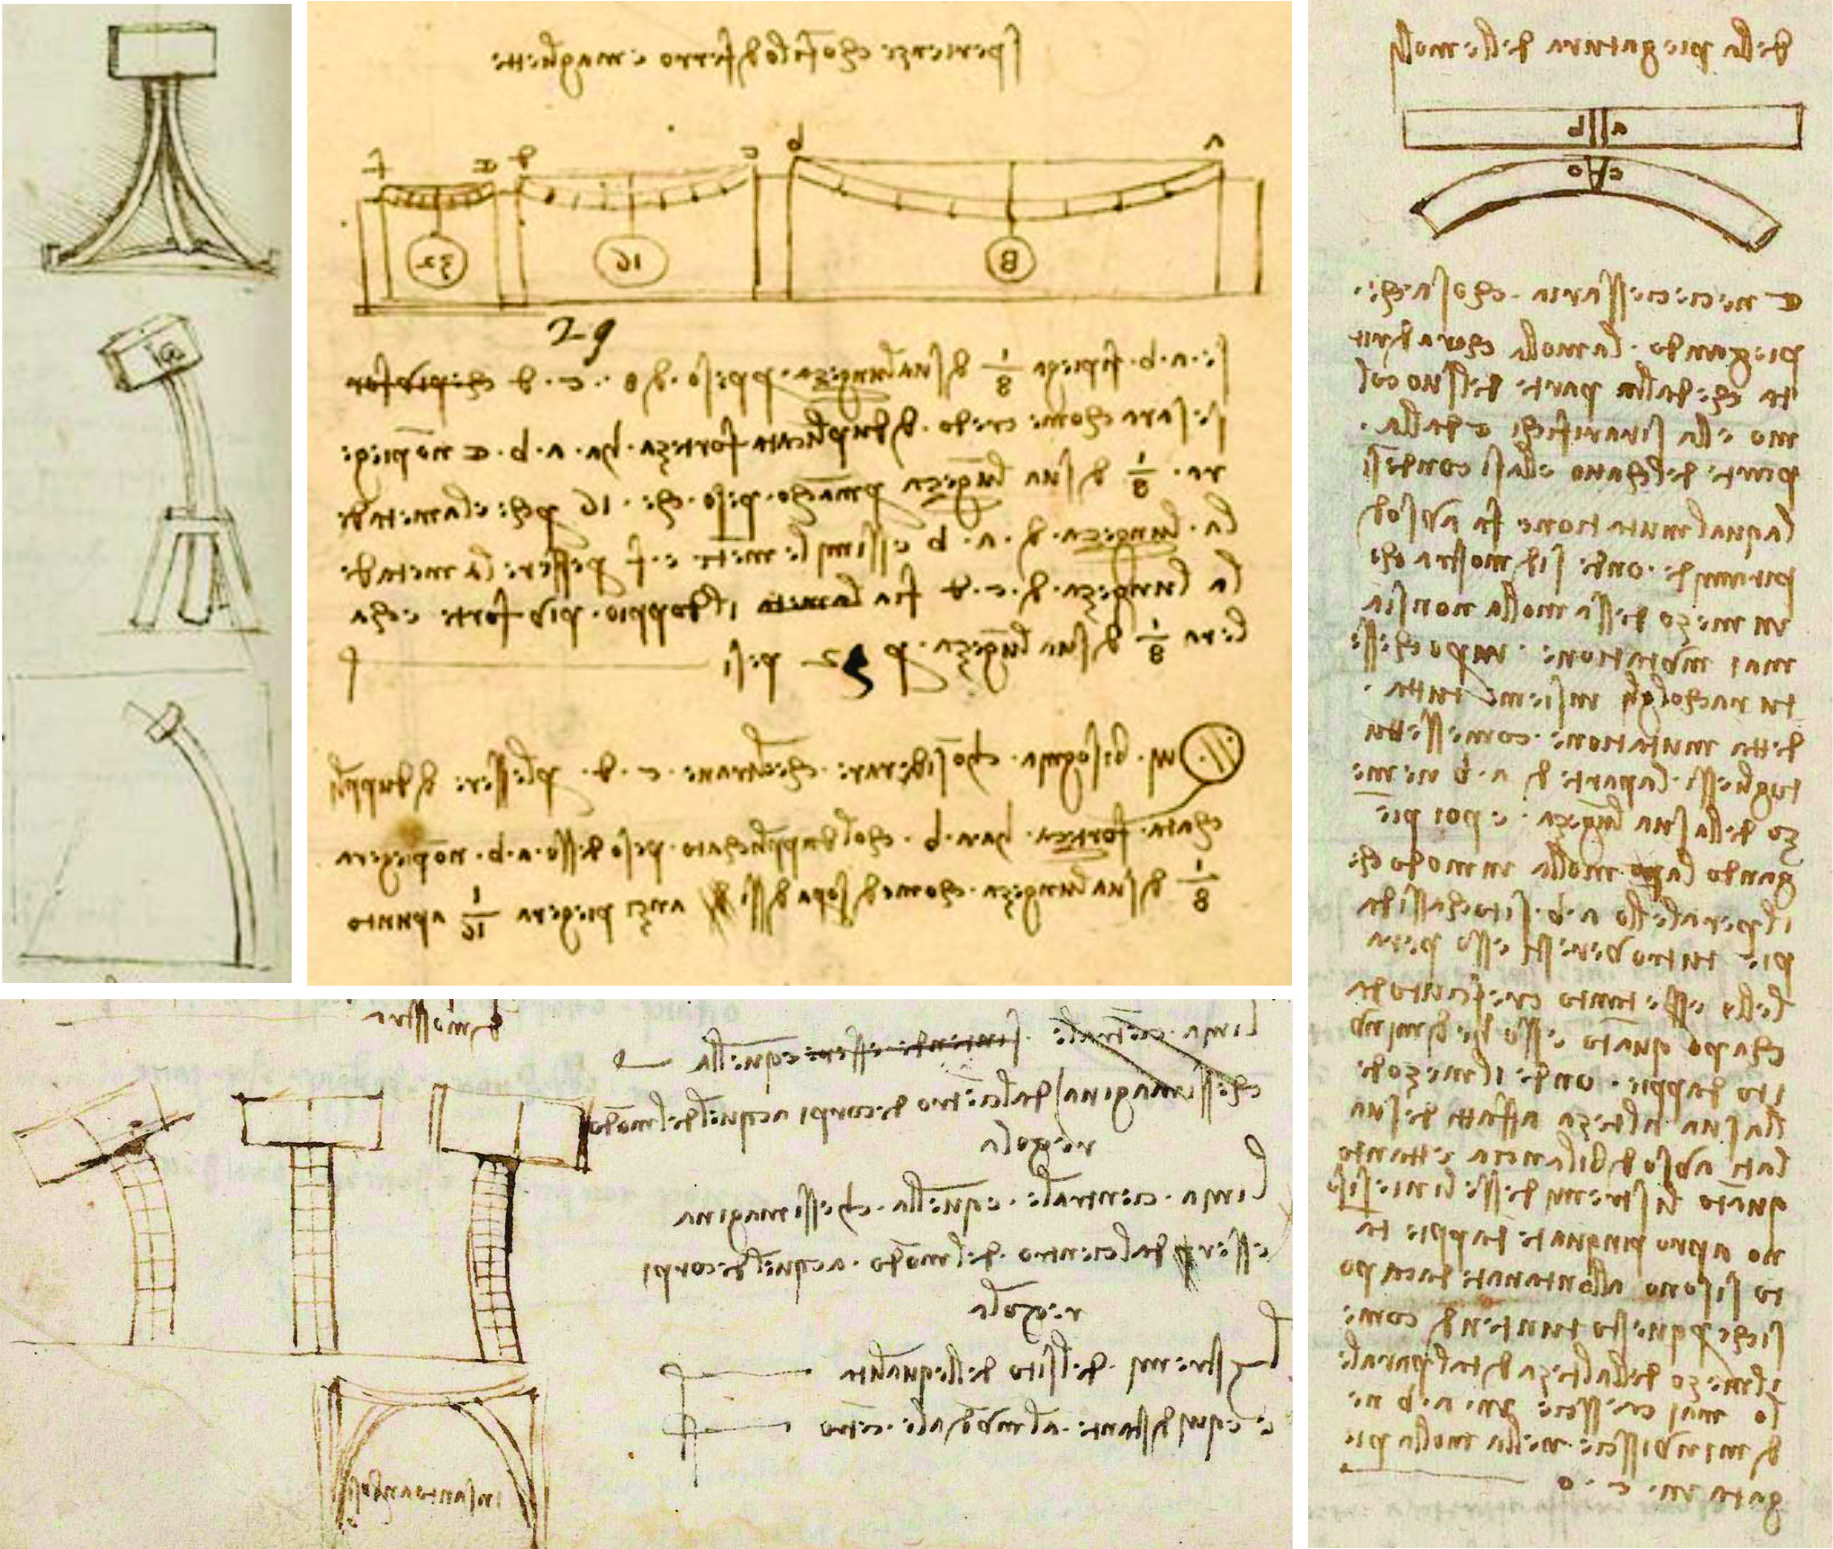
\includegraphics{partes/figs/Madrid84vAtl908r.jpg}}
	\end{center}
	\titfigura{Paris A f.45v, Atlanticus f.908r, Madrid I f.84v (right), 177v (bottom).}\label{fg:Madrid84vAtl908r}
\end{figure}
On figure \ref{fg:Madrid84vAtl908r}, some of these records are shown: sketches Paris A f.45v and Madrid I f.177v are studies on buckling of columns and the others are studies on bending of beams. In particular, the text on Madrid I f.84v, translated by \aut{Zammattio}\cite{zammattio_1980}, reads: \emph{``If a straight spring is bent, it is necessary that its convex part become thinner and its concave part, thicker. This modification is pyramidal, and consequently, there will never be a change in the middle of the spring. You shall discover, if you consider all of the aforementioned modifications, that by taking part `ab' in the middle of its length and then bending the spring in a way that the two parallel lines, `a' and `b' touch a the bottom, the distance between the parallel lines has grown as much at the top as it has diminished at the bottom. Therefore, the center of its height has become much like a balance for the sides. And the ends of those lines draw as close at the bottom as much as they draw away at the top. From this you will understand why the center of the height of the parallels never increases in `ab' nor diminishes in the bent spring at `co'.''} Moreover, the striking sketch on Codex Atlanticus f.222r, entitled \emph{Testing The Strength of Iron wires of Various Lengths}, shown in figure \ref{fg:Atl222r}, is the first known record on strength of materials. 
\begin{figure}[!ht]
	\centering
	\begin{center}
		\scalebox{.70}{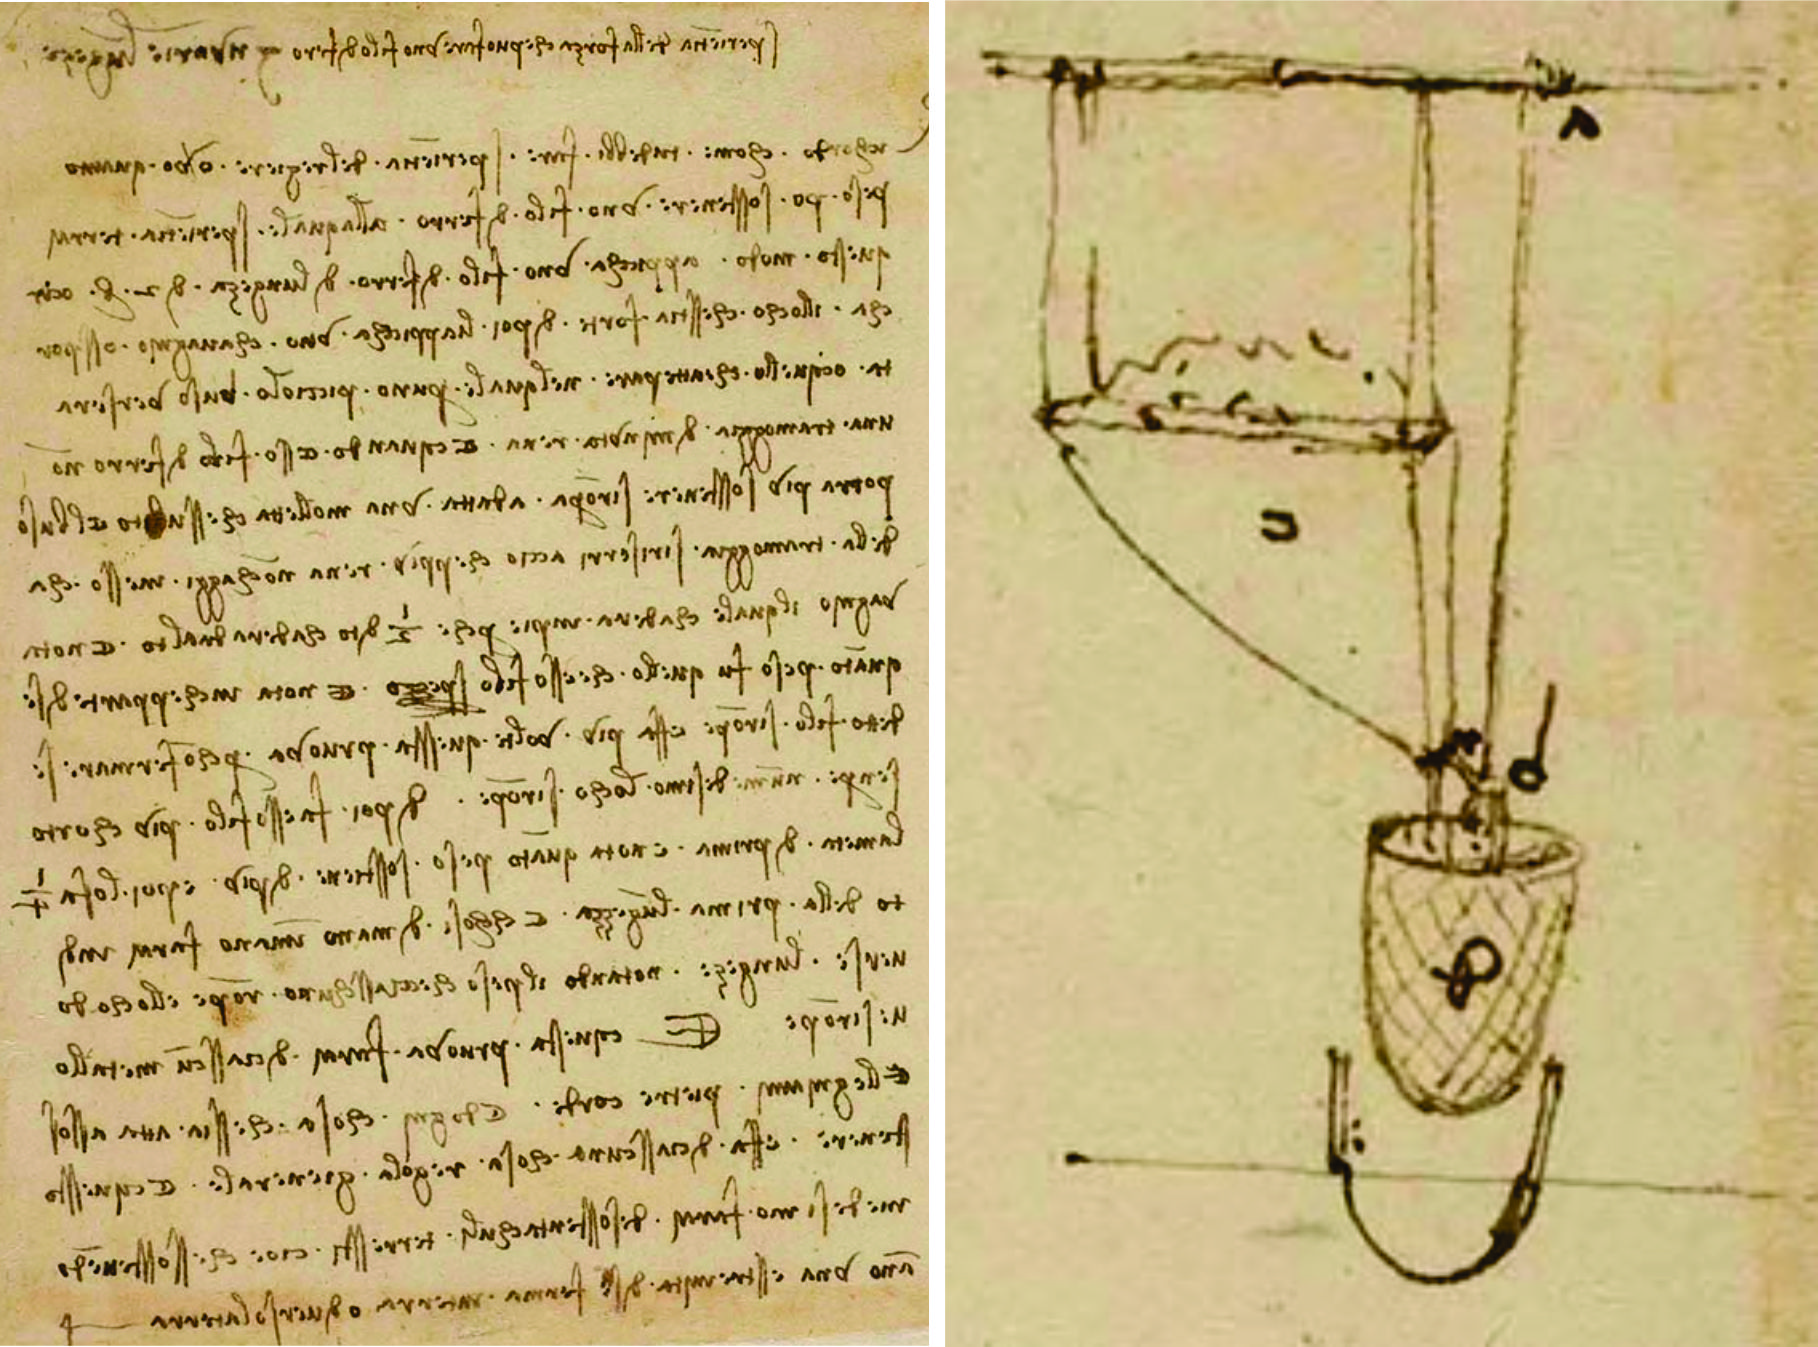
\includegraphics{partes/figs/Atl222r.jpg}}
	\end{center}
	\titfigura{Codex Atlanticus f.222r.}\label{fg:Atl222r}
\end{figure}
The drawing on the figure represents a test scheme of an iron wire with length `ab' and a given thickness. The wire suspends an initially empty basket `q' which is slowly loaded with sand by a hopper `c'. When the wire breaks, a spring closes the hopper and the basket falls a short distance into a hole, so as to not drop the sand. The sand in the basket is then weighted to obtain the strength of the wire. Still on this figure, an excerpt of the text reads: \emph{``The object of this test is to find the load an iron wire can carry. Attach an iron wire 2 braccia long to something which will firmly support it, then attach a basket or similar container to the wire and feed into the basket some fine sand through a small hole placed at the end of the hopper. A spring is fixed so that it will close the hole as soon as the wire breaks. The basket is not upset while falling, since it falls through a very short distance. The weight of sand and the location of the fracture of the wire are to be recorded. The test is repeated several times to check the results. Then a wire of 1/2 the previous length is tested and the additional weight it carries is recorded; then a wire of 1/4 length is tested and so forth, noting the ultimate strength and the location of the fracture.\footnote{\aut{Lund \& Byrne}\cite{lund_2000_1}, p.3.}''}       


Concerning the subject of Mechanics, which is our interest here, some scholars on the field contest the alleged scientific value of da Vinci's works: the most aggressive criticism is given by \aut{Truesdell}\cite{truesdell_1968}, which doubts, in his typical verbosity, whether da Vinci's sketches and annotations on engineering are really his creation or merely reproduce common technical knowledge of his time. Moreover, Truesdell argues that da Vinci's proposed physical laws, all of them linear, conceived intuitively from simple rules of three, are mostly wrong and the right ones just happened to be correct, since the laws in Physics are either linear or nonlinear. According to \aut{Dugas}\cite{dugas_1988_1}, da Vinci \emph{``...cuts the figure of a gifted amateur... He tackled all kinds of problem, often with more faith than success. Frequently he returned to the same problem by very different paths, and did not scruple to contradict himself.''} Therefore, from today's perspective, it is not possible to state that da Vinci's work on Mechanics directly anticipated relevant definitions or concepts on the field, despite his undeniable outstanding efforts as a curious and creative individual. But even if da Vinci's contributions were scientifically substantial, they would not serve as reference for the study of subsequent professional scholars because none of his notebooks was published in his time or shortly after his death.  


Unlike Leonardo da Vinci, his fellow countryman Galileo Galilei (1564-1642) received a formal education and, at the age of sixteen, enrolled the university of his hometown, Pisa, to study medicine. Among other disciplines, the course required knowledge on philosophy, provided by professors Francesco Buonamici and Girolamo Borro, as well as Mathematics and Astronomy, given by Father Filippo Fantoni, a monk. Both Buonamici and Borro were strict aristotelians, which meant that their teachings conflicted with the Christian dogmas of creationism, afterlife, immortality of the soul and others. Some biographers believe that this teachings intensified the impetuous spirit of Galileo, which would cause him trouble with fellow catholic academicians and also with the Inquisition years later. At a certain moment in 1583, Galileo attended lectures on Euclid's \emph{Elements} given by the former mathematician Ostilio Ricci, instructor at the Medici court. Amazed by the performance of the student, Ricci managed to convince Vincenzo Galilei, Galileo's father, to allow his son to switch from Medicine, which would assure a promising career, to Mathematics and Natural Philosophy, areas that captivated the young Galileo during his studies at the faculty. In 1585, following a not unusual practice among noble youngsters of his time, Galileu dropped out of the university, without a degree, in order to get a job: at Florence and Siena, he started private teaching his most interested subjects as a preparation for an eventual post of Mathematics professor on some important university. Meanwhile he kept attending the lectures of Ricci and also studying the work of other eminent mathematicians such as Giovanni Battista Benedetti, Christoph Clavius and Guidobaldo del Monte. In 1588, Galileo was invited to lecture at the Florentine Academy about the location and dimensions of the hell in Dante's \emph{Inferno}\footnote{See \aut{Wallace}\cite{wallace_1998_1}.}. The favorable impressions that these lectures caused on the tuscan nobility and the quitting of Father Fantoni, as well as recommendations from professor Clavius and other mathematicians, enable Galileo to get a chair on Mathematics at the University of Pisa in 1589. After three years of professorship in Pisa, Galileo was convinced by the fellow Medicine professor Girolamo Mercuriale to apply for a vacant chair on Mathematics at the University of Padua, which paid three times more than Pisa. Starting in December 1592, he worked at Padua for eighteen years and then returned to Florence as a mathematician of the Medici court.    

During his Padua years, which he considered the happiest of his life, Galileo developed his most notable works, particularly on Kinematics and Astronomy. He also endeavored to develop studies on strength of materials, which would be published in \emph{Dialogs Concerning Two New Sciences} forty years later. From this book, whose dialogs between characters Salviati, Sagredo and Simplicio occur during four days, it is noteworthy for our purposes to present the  attempt of Galileo to calculate the strength of cantilever beams. On the second day, Salviati proposes a solution to the problem depicted on the right in figure \ref{fg:galileo}. 
\begin{figure}[!ht]
	\centering
	\begin{center}
		\scalebox{.72}{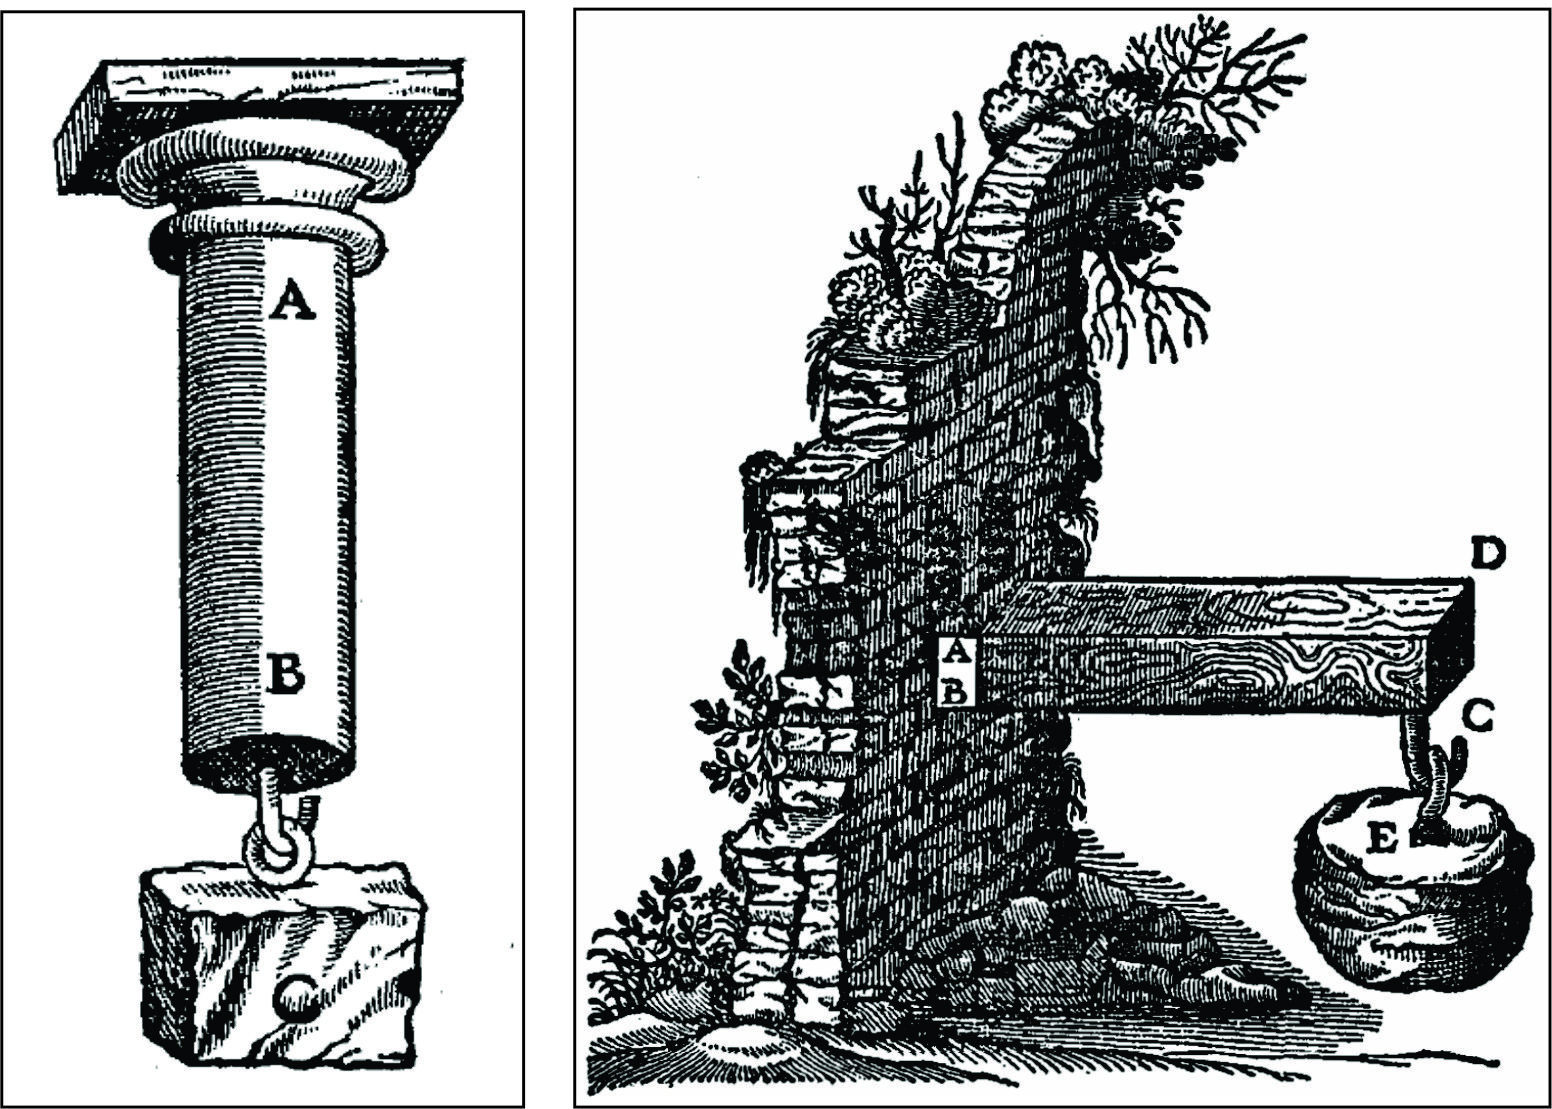
\includegraphics{partes/figs/galileo.jpg}}
	\end{center}
	\titfigura{Beams in tension and bending (\aut{Galileo}\cite{galileo_1954_2}).}\label{fg:galileo}
\end{figure}
He says to his interlocutors that ``\emph{the \emph{momento} of the force applied at C bears to the \emph{momento} of the resistance, found in the thickness of the prism, i. e., in the attachment of the base BA to its contiguous parts, the same ratio which the length CB bears to half the length BA; if we now define absolute resistance to fracture as that offered to a longitudinal pull -- \emph{[drawing on the left in previous figure]}... then it follows that the absolute resistance of the prism BD is to the breaking load placed at the end of the lever BC in the same radio as the length BC is to the half of AB, in the case of a prism, or the semidiameter in the case of a cylinder}.\footnote{\aut{Galileo}\cite{galileo_1954_2}, p.115.}'' In other words, if we call $h$ the thickness of the prism, $\tau_u.h.AB$ his ``absolute resistance to fracture'' and $E_u$ his ``breaking load'', then Salviati states that 
\begin{eqnarray*}
\dfrac{\tau_u.h.AB}{E_u}=\dfrac{BC}{AB/2}&\text{or}&E_u=\dfrac{\tau_u.h.AB^2}{2.BC}\,.
\end{eqnarray*}
But if Simplicio and Sagredo were more argumentative and cautious, they would verify this categoric statement and would see that Salviati's proposal is dangerously wrong for the case of beams made of steel: the ultimate load for rectangular cross sectional cantilever steel beams on pure bending is actually three times less\footnote{See \aut{Popov}\cite{popov_1990_1}, p.286.} than $E_u$. When Salviati specifies a \emph{momento} from a load with an arm $AB/2$ that balances the \emph{momento} of the lever BC caused by $E$, he inadvertently defines that the tensile load distribution on section $AB$ is uniform and that there is a longitudinal compressive load concentrated at fulcrum $B$ in order to balance this tensile load distribution. The reasons that made Galileo arrive at this conclusion are subject of debate: \aut{Higdon et al}\cite{higdon_1981_3} speculate that he might have observed the failure of bending beams made of stone. On brittle materials like this, the shape of the fracture caused by axial loads and pure bending are very similar, which probably induced him to wrongly consider an axial resistance on the bending beam. Since Galileo was the first to formally address the problem of the strength of a cantilever beam subjected to pure bending, it is commonly known as \textsb{Galileo's Problem}\index{Galileo!Problem}\footnote{See \aut{Benvenuto}\cite{benvenuto_1991}, p.177.}. 

The French scholar Edm\'e Mariotte (?-1684) also contributed to the mechanics of deformable bodies, but he is best known for his work on the properties of air, entitled \emph{Discourse on the Nature of Air}, published in 1676, in which he proposed the notorious inverse relation between volume and pressure: today, we call it the Boyle-Mariotte Law for gases. The early life of Mariotte is completely unknown and the first registered document of his existence is a letter he sent from Dijon in 1668 to the dutch physicist Christiaan Huygens, where he announced the discovery of the blind spot in human eye. It is also unclear how the Paris Academy of Sciences became acquainted with Mariotte's works on plant physiology, but the excellent impression that he caused on the academicians when invited to go to Paris in order to present his theories and experiments soon enabled his engagement at the Academy on 27 July 1667, as a \emph{physicien}. Following a usual practice of the scholars of his time, Mariotte wrote articles on a great variety of subjects: Mathematics, Mechanics, Astronomy, medicine, hydrology, musical theory, plant biology, among others. His body of published work is extensive and the most important texts are the following: four essays, gathered under the title \emph{Essays on Pshyics}, of which the already mentioned \emph{Discourse on the Nature of Air} is part; a \emph{Treatise on the Motion of Water and Other Fluid Bodies}, published unfinished and postumously in 1686, where Mariotte studies natural springs, artificial fountains and the flow of water through pipes; and a \emph{Treatise on the Collision or Shock of Bodies}, first published in 1673, which covers the topic of elastic and inelastic collisions and shows Mariotte's abilities as a gifted experimenter. It is important to account that Mariotte's work heavily relied on the subjects commonly studied and produced by others at the Paris Academy and, apart from the volume-pressure relation, there is no relevant discoveries attributed to him. However, since rigorous and exhaustive experimentation is the fundamental basis of his efforts, some authors recognize him as the man who introduced the experimental physics into France. In corollary 6 of his third law of motion, \aut{Newton}\cite{newton_1999_1} cites Mariotte's book on collisions: ``\emph{But Wren additionally proved the truth of these rules before the Royal Society by means of an experiment with pendulums, which the eminent Mariotte soon after thought worthy to be made the subject of a whole book.}''
  

In part V of his \emph{Treatise on the Motion of Water and Other Fluid Bodies}, called \emph{On Water Motion and Pipe Strength}, Mariotte undertakes the study of Galileo's Problem in order to correctly design the dimensions of water pipes because he verified experimentally that Galileo's proposition of an axial strength on the bending beam was incorrect for the case of iron and wood. On the discourse II of this same part V, he starts by specifying that the axial strength of a beam will be measured not by a maximum load (absolute resistance to fracture), but by a maximum extension: the beam performs a certain extension in order to sustain a certain load; there is then a maximum extension over which the beam breaks. This is the first known quantitative consideration of deformation in the study of the resistance of deformable bodies. Still in part V, discourse II, Mariotte also describes in literal form a load-extension relation: ``\emph{... if a solid of wood needs to extend two lines to break, and a weight of 500 pounds make this extension, a weight of 125 pounds make it extend about half a line, 250 pounds, about one line, etc. Thus, each extension will balance with a certain weight.}\footnote{\aut{Benvenuto}\cite{benvenuto_1991}, p.266.}''. The drawing on the left in figure \ref{fg:mariotte} is a model conceived by Mariotte to study the behavior of the material fibers of a cantilever beam using identical chords $DI$, $GL$ and $HM$ subjected to tension by a lever $N$ with a given fulcrum $C$.     
\begin{figure}[!ht]
	\centering
	\begin{center}
		\scalebox{.72}{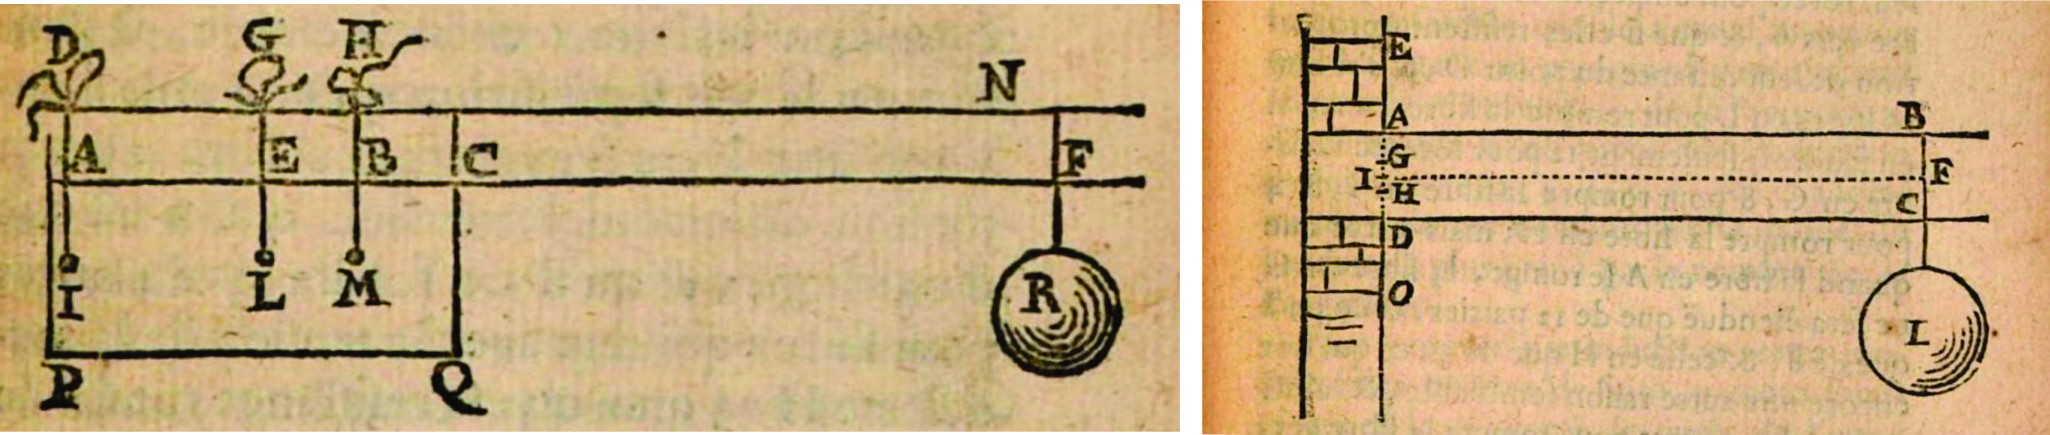
\includegraphics{partes/figs/mariotte.jpg}}
	\end{center}
	\titfigura{Extension of chords and Galileo's Problem (\aut{Mariotte}\cite{mariotte_1740_1}, pp.353-355).}\label{fg:mariotte}
\end{figure}
The rectangle $ACQP$ represents the part of the cantilever, shown on the right in this same figure, that is inside the wall and $AC=2.EC=4.BC$. Mariotte then measured the extensions $\epsilon_{DI}$, $\epsilon_{GL}$ and $\epsilon_{HM}$  of the chords until rupture for different applied loads $R$ and observed the relation $\epsilon_{DI}=2.\epsilon_{GL}=4.\epsilon_{HM}$, which is the same for the loads on the chords, assuming his load-extension law. For an infinite number of chords, the load distribution on face $AC$ decreases linearly to zero from $A$ to $C$ and therefore the resultant load acts at a distance $AC/3$ from $A$. Now considering the drawing on the right in figure \ref{fg:mariotte}, from his extensive experiments, Mariotte came to the conclusion that the beam fibers on the face $AD$ under the middle point $I$ are in compression and the fibers over $I$ are subjected to tension. These fibers in tension behave just like the chords of his model, that is, their extension decreases linearly to zero, from $A$ to $I$, and the resultant load\footnote{Points $G$ and $H$  do not refer to $AI/3$ and $DI/3$ but to another development by \aut{Mariotte}\cite{mariotte_1740_1}.} is at $AI/3$ from $A$. For the compressed fibers, Mariotte considered the same triangular distribution from his model of chords, applied to compressive loads, and thus the resultant compressive load is at $DI/3$ from $D$. He then considers that ``\emph{these extensions and these compressions will share the force of the weight $L$: adding one third of the thickness $IA$ to the third of the thickness $ID$, the whole will be equal to one third of the whole thickness $AD$; from which the same thing will follow as if all the parts extended.}\footnote{\aut{Benvenuto}\cite{benvenuto_1991}, p.268.}'' Since Mariotte did not express this vague reasoning in a literal or mathematical expression for the breaking load, it is at least improper to attribute to him the incorrect triangular distribution of loads on face $AD$, as is usually done. Despite the imprecision of Mariotte's proposition, we dare to interpret it as follows: the resistance of the extended fibers corresponds to half of the total resistance of the beam. In this context, isolating the upper part $AI$, we must consider a compressive longitudinal load concentrated on $I$ in order to balance the tensile loads on face $AI$. Thereby, let the beam be a prism, just like the case of Galileo's Problem, $h$ its thickness, $\tau_u.h.AD$ is Galileo's absolute resistance to fracture, $L_u$ the breaking load. The balance of \emph{momenta} relative to fulcrum I is  
\begin{eqnarray*}
\frac{L_u}{2}.DC = \frac{\tau_u.h.AD}{2} \dfrac{2.AI}{3}&\text{or}&L_u=\dfrac{\tau_u.h.AD^2}{3.DC}\,,
\end{eqnarray*}
which results in a breaking load two times greater than the ultimate load for rectangular cross sectional cantilever steel beams subjected to pure bending. 

Regarding his load-extension law, described previously, it is improbable that Mariotte knew the \emph{Lectures \emph{de Potentia Restitutiva} Or of Spring}, written by the member of the Royal Society of London Robert Hooke (1635-1703) and published in 1678, eight years before Mariotte's treatise on fluids. In this book, Hooke's approach on material deformation is broader than his French contemporary's: a linear load-extension law is presented as part of a general constitutive property of ``springing bodies'', as classified by him to express the behavior of deformed bodies that recover their initial shape after load removal, a feature currently known as elasticity. But before exploring this work, let's learn a little about its author's life. Hooke was born at the village of Freshwater, a peninsula on the west of the English Island of Wight, on July 18 and baptized eight days later by his own father, John Hooke, minister of that remote Anglican parish. Because of a weak constitution and recurrent illnesses until the age of seven, the family doubted Hooke would survive beyond childhood. After this period, but still suffering from frequent headaches, the boy did not show interest on the religious studies oriented by his father and preferred to spend most of hist time building mechanical toys. After his father's death in 1648, when he inherited a small sum of money, there are no records of Hooke's life until the age of twenty, when he went to live at the house of Richard Busby, the headmaster of the Westminster school. There, he became proficient on Latin and Greek, as well as Hebrew and other oriental languages. Under Busby orientation, he mastered Euclid's Elements by himself, ``\emph{and thence proceeded orderly from that sure Basis to the other parts of the Mathematicks, and after to the application thereof to Mechanicks, his first and last Mistress.}\footnote{\aut{Hooke}\cite{hooke_1705_1}, p.iii.}'' In 1653, he became a student of the Christ-Church, a constituent college of the University of Oxford, and received the degree of Master of Arts in 1662 or 1663. During this period at the college, he first worked as assistant to the medicine professor Dr. Thomas Willis and then to the eminent natural philosopher Dr. Robert Boyle from 1655 to 1662. In order to drive a pneumatic engine designed by Boyle, which enabled the publication of the famous Boyle's Law on gases (the same as Mariotte's) in 1662, Hooke contrived and perfected an air pump. In this same period, he attempted designs of structures attached to the human body in order to enable flying, but concluded that it was impossible because human muscles were not strong enough for the task. He took active part on the meetings with the group of scholars that would soon found the Royal Society of London in 1660. Already member of the Royal Society and famous for his incomparable skills as a mechanical experimenter, Hooke was nominated the curator of experiments of the Society in November 1661 and could take up his post with the blessings of Boyle, who released him. On the beginning, Hooke was in charge of providing every weekly meeting of the Royal Society with some new experiment or practical presentation on Mechanics, his expertise. However, since specialization at that time was not a virtue, Hooke published in 1665 the first relevant book on biological microscopic observations called \emph{Micrographia}, to which he built his own microscope and where the term ``cell'' was coined to refer to small biological structures. The following year, after the great fire of London, Hooke was appointed one of the surveyors to rebuild the city and was heavily demanded as an architect, which assured him a substantial financial income for the following ten years. During this period, the most productive of his career, Hooke kept working at the Society, giving lectures and publishing papers: the aforementioned \emph{Lectures \emph{de Potentia Restitutiva} Or of Spring} is one of them. 


In a very pragmatic style, Hooke does not waste time with preambles and at the very beginning of these lectures on springs, he starts describing the famous load-extension law that would bare his name until today: ``\emph{About two years since I printed this Theory in an Anagram at the end of my Book of the Descriptions of Helioscopes, \emph{viz, ceiiinosssttuu, id est, Ut tensio sic vis}; That is, the Power [force] of any Spring is in the same proportion with the [ex]Tension thereof: that is, if one power [force] stretch or bend it one space, two will bend it two, and three will bend it three, and so forward... And this is the Rule or Law of Nature, upon which all manner of Restituent or Springing motion does proceed... It is very evident that the Rule or Law of Nature in every springing body is, that the force or power thereof to restore itself to its natural position is always proportionate to the Distance or space it is removed therefrom...\footnote{\aut{Hooke}\cite{hooke_1678_1}, pp.1,2,4.}}'' In mathematical words, for each pair of applied load $F_i$ and extension $x_i$, value $k=F_i/x_i$ is a constant that is constitutive of the spring. Thereby, \textsb{Hooke's Law}\index{Law!Hooke's} can be described as the following: in other to attain an arbitrary extension $x$ of a spring with constant $k$, the applied force needs to be 
\begin{equation}
F=kx\,,
\end{equation}
and thus the restitutive force of the spring is obviously $-kx$. It is common to assume that when the spring is stretched, $x$ is positive; when compressed, it is negative. In the cited paragraph, Hooke also states that the load-extension relation of every springing body (elastic beam) is always linear, but this is incorrect since not all elastic bodies behave linearly. Therefore, in the context of elasticity, a body is called \textsb{Hookean}\index{body!Hookean} when it observes Hooke's Law, that is, when it deforms linearly. Figure \ref{fg:hooke} illustrates the two springs built by Hooke to obtain the results for his Law.  
\begin{figure}[!ht]
	\centering
	\begin{center}
		\scalebox{.72}{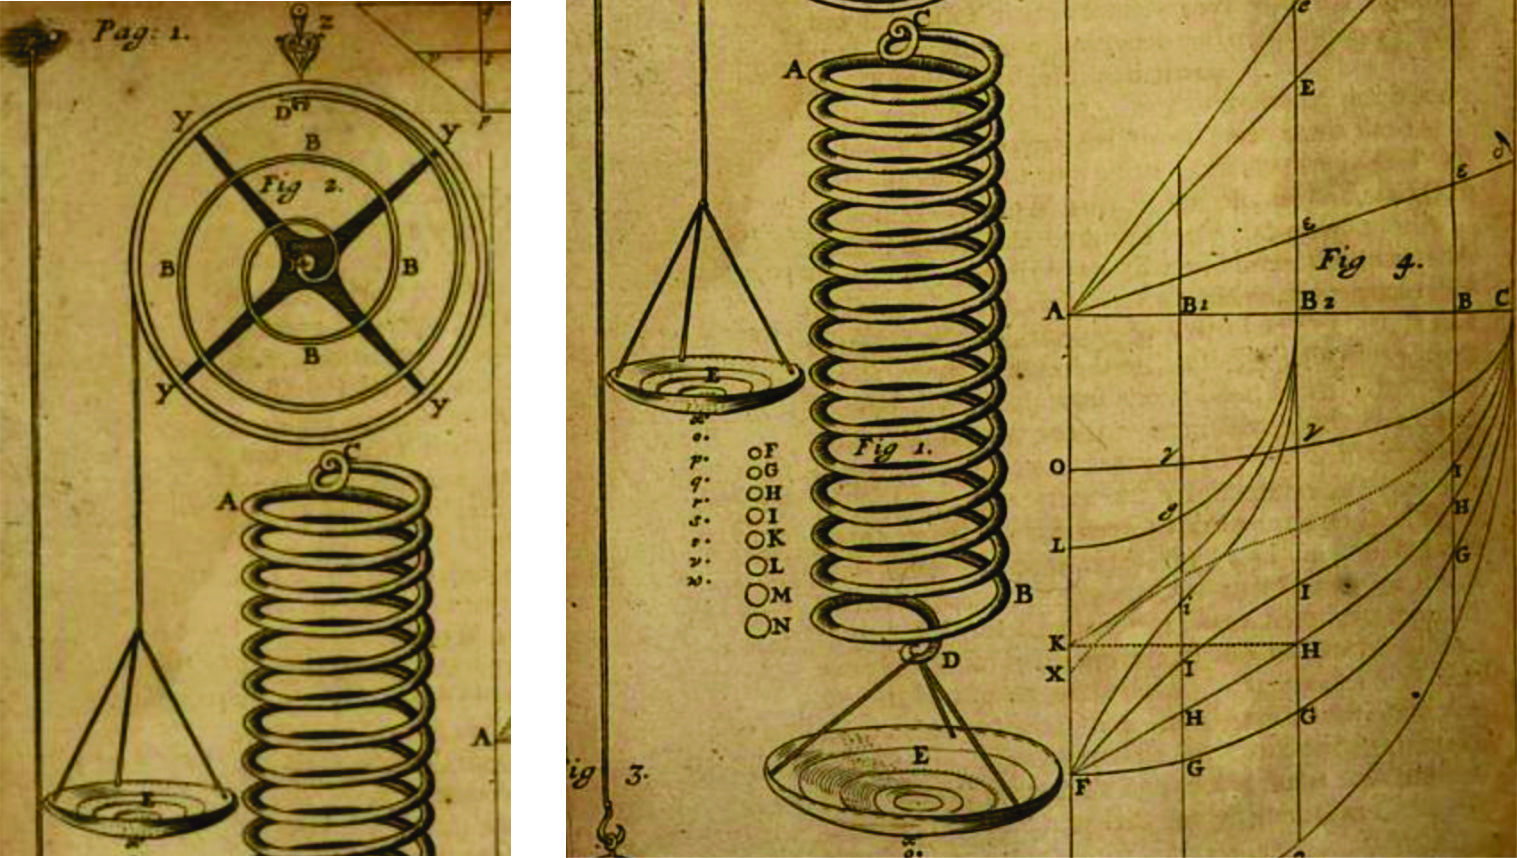
\includegraphics{partes/figs/hooke.jpg}}
	\end{center}
	\titfigura{Springs built by \aut{Hooke}\cite{hooke_1678_1} for his Law.}\label{fg:hooke}
\end{figure}

Concerning Galileo's Problem, Hooke did not apply his theory of springing bodies to solve it, but only to describe a ``compound way of springing\footnote{\aut{Hooke}\cite{hooke_1678_1}, p. 15.}'', resulting from the curvature of the deformed cantilever, where its inner elastic fibers are compressed and the external are stretched. Speaking of curvature, the mathematical description of the deflection or curvature of bending beams was first addressed by the swiss mathematician Jakob Bernoulli (1654-1705) on an article\footnote{See \aut{Truesdell}\cite{truesdell_1960}, p. 89.} in 1694, a study he called the problem of the \emph{curvatura laminae elasticae} (elastic band curvature), or simply \textsb{\emph{elastica}}\index{elastica}. Born in the city of Basel, Jakob was the eldest son of pharmacist Nikolaus Bernoulli and Margaretha Sch\"onauer, daughter of a banker. Nikolaus's father, also Jakob Bernoulli, was a merchant and emigrated from Amsterdam to Basel, where he became a swiss citizen through marriage. Jakob received his master of arts in philosophy in 1671 and, compelled by his father, graduated in theology in 1676, both at the University of Basel; but, to his parents dismay, during these university years, Jacob became strongly interested in Mathematics and astronomy. In the same year of 1676, working as a tutor of nobles, he traveled to Geneva and then to France, where he lived for two years and could study the works of Descartes and followers. From 1681 to 1682, Jakob resumed his travels, but this time to make contact with scholars and mathematicians in Holland and England, where he met Robert Boyle and Robert Hooke. Back to Basel, during 1683, he started giving lectures on Mechanics and also publishing articles on Geometry and Algebra in the prominent scientific periodicals \emph{Journal des S\c{c}avans} and the \emph{Acta Eruditorum}. In 1684, Jakob married Judith Stupanus, daughter of a pharmacist, with whom he had two children. He kept working and publishing on Mathematics, as well as exchanging an intense scientific epistolary correspondence with acquaintances he made during his travels, including Leibniz, Huygens and others. In this period, his brother Johann Bernoulli (1667-1748) was studying medicine at the university, also compelled by Nikolaus, but Johann secretly started studying Mathematics by himself, under the orientation of Jakob. After the appointment of Jakob as professor of Mathematics at the University of Basel in 1687, both brothers started studying the differential calculus of Leibniz and adopted his differential notation for derivatives, that is, they became ``Leibnizians'', as opposed to british ``Newtonians'', who worked with Newton's fluxions and fluents, concepts that embodied the infinitely small number $o$. In a paper published in the 1690 edition of \emph{Acta Eruditorum}, concerning the solutions of the problem of the catenary curve proposed by Huygens and Leibniz, Jakob coined the term ``integral'' in the sense we currently use. Among his works, the main contributions deal with problems and propositions on Calculus, Probability and Series. According to \aut{Maugin}\cite{maugin_2014}, Jakob ``\emph{may have been less creative than John [Johann], but nonetheless played an essential role in the dissemination of integral calculus ..., in the establishment of the theory of probabilities, and in solving critical problems in mechanics (the isochronous curve, the \emph{elastica}).}''  

From 1690 to 1695, Jakob decided to study the so called flexible lines; mainly the catenary, the isochronous curve and the \emph{elastica}. Our interest here is his contribution on the deflection and curvature of the \emph{elastica}, which is an elastic band deformed by its own weight or by a weight or couple applied to one or both of its endings. Jakob had referred to the problem of the \emph{elastica} with an ending fixed and the other deflected by a load, proposed by Leibniz in private letters, in an article published 1691, announcing that he would present a solution the following year\footnote{See \aut{Truesdell}\cite{truesdell_1960}, p. 88.}; but it took three years until \emph{Curvatura Laminae Elasticae, \&c.} was finally submitted to \emph{Acta Eruditorum}. Jakob starts this article by saying that ``\emph{After a silence of three years I keep my word; but in such a way as right richly to compensate for that delay, which else the reader might have borne with annoyance, since I exhibit the curvature of springs not in one way only (as I had promised in the beginning) but generally for any hypothesis on the elongations; which, unless I err, I am the first to achieve, after the problem was attempted in vain by many.}\footnote{\aut{Jakob Bernoulli}\cite{jakob_1694}, pp. 262-263, translated from the Latin by \aut{Truesdell}\cite{truesdell_1960}.}'' In order to understand what he did, we reproduce on figure \ref{fg:jakob} one of the diagrams presented in the article.     
\begin{figure}[!ht]
	\centering
	\begin{center}
		\scalebox{.70}{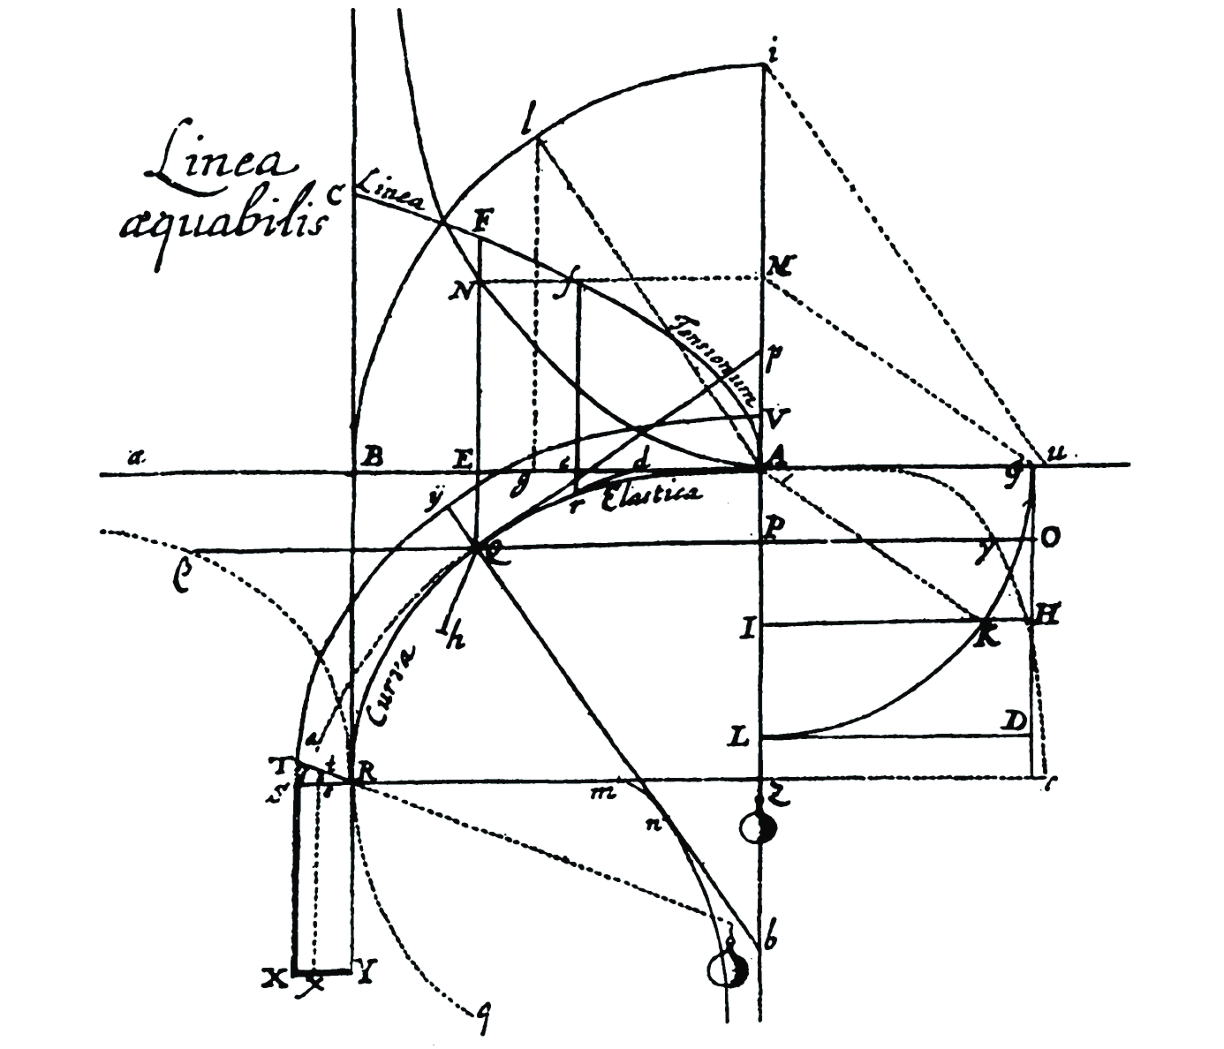
\includegraphics{partes/figs/jakob.jpg}}
	\end{center}
	\titfigura{Study on the \emph{curva elastica} by \aut{Jakob Bernoulli}\cite{jakob_1694}.}\label{fg:jakob}
\end{figure}
Fixed to the support $SRYX$, he draws a beam $SVAR$ with uniform rectangular section, the inner fiber of which is the \emph{elastica} to be studied. The beam sustains a weight Z, whose chord is perpendicular to the tangent $au$ on $A$. The curve $AC$ represents the load-extension relation at an arbitrary point $y$, where the load, on the abscissa, increases from $A$ to $B$ and the extension increases from $B$ to $C$. And that's it: with the help of the shape and proportions of the geometry presented, the reader is supposed to understand and accept that the curvature $\kappa:=1/Qn$ at point $Q$ is directly proportional to distance $QP$. The year following the publication of this article, Jakob submitted another to the same periodical, making things clearer: ``\emph{I consider a lever with fulcrum $Q$, in which the thickness $Qy$ of the band [beam] forms the shorter arm, the part of the curve $AQ$ the longer. Since $Qy$ and the attached weight $Z$ remain the same, it is clear that the force [load] stretching the filament [fiber] at $y$ ... is proportional to the segment $QP$.}\footnote{\aut{Jakob Bernoulli}\cite{jakob_1695}, p. 538, translated from the Latin by \aut{Truesdell}\cite{truesdell_1960}.}'' In other words, he assumes that the moment $QP.Z$ is balanced by $Qy.F$, where $F$ represents the load that stretches $y$ an extension $e$, measured relative to initial length of the \emph{elastica} $AR$. Since $Qy$ and $Z$ are constants, $F$ is directly proportional to $QP$. Moreover, since $F$ is directly proportional to $e$, according to his load-extension relation, then $e$ is directly proportional to $QP$; but since $e$ is inversely proportional to $Qn$, then $k$ is directly proportional to $QP$. Mathematically, equality $Qy.F=QP.Z$ implies that $QP \propto F \propto e \propto 1/Qn$. Then, Jakob proposed that 
\begin{equation*}
\kappa=\dfrac{e}{Qy}
\end{equation*}
and, knowing the formula for the curvature of a plane curve, called by him the ``golden theorem'', he arrived at an equation of the deflection\footnote{See \aut{Truesdell}\cite{truesdell_1960}, p. 93.}. However, for some strange reason, Jakob incorrectly considered only the moment $Qy.F$ to balance $QP.Z$ and not the moment correspondent to the whole distribution of forces in section $Qy$, a distribution he studied because lines $ST$ and $st$ are drawn to represent the elongations of two different points on the cross section $RS$. 


With fundamental studies on differential equations, Calculus of Variations and other problems of Mathematics, the ``more creative'' brother Johann is considered to be the most brilliant mathematician of the Bernoulli dynasty on this field\footnote{See \aut{Maugin}\cite{maugin_2014}, p. 8.}. From his early studies on medicine, Johann defended in 1694 one the first known doctoral thesis on biomechanics, where he described the motion of muscles. It would be incorrect to say that he did not specifically contribute to the subject of deformable bodies: besides introducing the concept of  what today is known as the principle of virtual work in a letter to the French mathematician Pierre Varignon (1654-1722) in February 26th, 1715, Johann is the father and master of Daniel Bernoulli (1700-1782), who, among other notable works, substantially developed and generalized the ideas of his uncle Jakob on the \emph{elastica}. The second son of Johann Bernoulli and Dorothea Falkner, Daniel was born in the dutch city of Groningen, when his father held a post of Mathematics professor at the university. At the age of thirteen, with the family already living at Basel, Daniel was sent to the university to study philosophy and logic. During this time, he also studied Mathematics privatley, oriented by his father and his elder brother Nikolaus. However, when Daniel finished his studies in 1716, Johann determined he would be a merchant and sent him to learn the profession. Daniel showed enough evidences that he had no talent for commercial business and finally expressed his wishes to study Mathematics, but Johann strongly disagreed, arguing that Mathematics did not bring financial comfort. A compromise solution was found and Daniel ended up enrolling at the University of Basel to study medicine, while keeping his private studies in Mathematics and Physics. As a result, and just like his father Johann, Daniel defended a thesis on biomechanics, more specifically on the mechanics of breathing, when he completed the medicine course in 1721. In order to follow an academic career at Basel, Daniel applied firstly for a chair on anatomy and botany and secondly for a vacant chair on logic, but both chairs were defined by lottery, which he lost out. Disappointed by this bad luck, Daniel went to Venice in order to practice medicine, but did not abandon Mathematics, and published a book entitled \emph{Exercitationes Quaedam Mathematicae} in 1724, with the help of German mathematician Christian Goldbach (1690-1764). The work presents four ``exercises'': a probabilistic description of a game; a discussion on the flow of water in a hole, which was incorrect; a study on differential equations; and a study on geometry of circular figures. His medical studies on blood flow greatly influenced his second exercise, which would stimulate him to keep studying the motion of fluids. Although \emph{Exercitationes} did not make any new or relevant contribution, it enabled the name of Daniel Bernoulli to be known in scientific circles. When his father Johann dropped an offer for a chair at the Imperial Academy of Sciences and Arts in St. Petersburg on behalf of him, the name of Daniel was immediately accepted. He assumed the chair of Mathematics at the Academy in 1725, together with his elder brother Nikolaus, a condition previously imposed by Daniel to accept the arrangement of his father. Eight months after their arrival at St. Petersburg Nikolaus died, a personal tragedy that affected Daniel in such a way that made him write to his father communicating his intentions to return to Basel. In order to alleviate Daniel sadness and also to help the young Leonhard Euler (1707-1783), Johann arranged a way to make his outstanding pupil be accepted to work with his son at the Imperial Academy. Euler arrived at St. Petersburg in 1727 and until Daniel return to Basel in 1733, they collaborated intensely and proficuously. In this period, Daniel and Euler produced fundamental contributions to the vibration theory, probability and political economy, as well as the mechanics of elastic and flexible bodies. Still in St. Petersburg, Daniel developed and finished his most notable work, which he would publish only in 1738, called \emph{Hydrodynamica}. In this book, the conservation of energy, conceived by his father, where an isolated body in motion balances kinetic and potential energies, is the base for  a particular version applied to fluids, the famous Bernoulli's principle, which states, in current terminology, that an isolated fluid in incompressible flow (reversible and adiabatic process) balances kinetic energy and static pressure. Moreover, according to \aut{Mikhailov}\cite{mikhailov_2005}, in this work Daniel also ``\emph{develops the first model of the kinetic theory of gases, approaches the principle of conservation of energy, establishes a foundation for the analysis of efficiency of machines, and he develops a theory of hydroreactive (water-jet) ship propulsion, including a solution of the first problem of motion of a variable-mass system.}'' From 1731 on, Daniel began applying for posts at the University of Basel, but he only got the chair of botany, which was a sufficient reason for him to leave St. Petersburg in 1733. Already at home, Daniel submitted a study on astronomy to the Grand Prize of the Paris Academy in 1734; a prize to which Johann had also submitted a similar work. The fact that father and son were declared joint winners led to strong quarrels between them and the relationship, which had always been full of tension and envy, suffered a definitive break up. After this event, Daniel never again developed himself any relevant mathematical work, although he kept an active correspondence and collaboration with Euler, that stayed in St. Petersburg.

In the Bernoulli-Euler epistolary collaboration on the study flexible lines, including statical and vibrational behaviors, Daniel acted mainly as an instigator, proposing problems and suggesting directions to follow, while Euler conceived brilliant solutions, definitions, methods and generalizations; in other words, Daniel oriented and Euler made it happen, beautifully. But before we describe their great contribution to the mathematical description of elastic bands, which is our concern here, we request the reader to indulgently follows us now through some words about Euler the man. First-born child of the calvinist pastor Paulus Euler and Margaretha Brucker, daughter of a hospital vicar, the swiss mathematician Leonhard Euler was born in Basel, from where the family moved when he was around one year old due to the appointment of his father to be the minister of a parish in the nearby town of Riehen. Paulus had enrolled the University of Basel back in 1685 and chose protestant theology to be his field of study. During the initial semesters, in October of 1688, to be precise, he attended a course on geometry and algebra given by the renowned mathematician Jakob Bernoulli, whose family Paulus became acquainted with. This course on Mathematics, whose final work was a thesis on Algebra he had to defend, probably inspired Paulus to tutor the young Euler on the first elementary algebraic concepts, and then \emph{Algebra}, written by the German mathematician Christoff Rudolff (1499-1545), was adopted as a textbook. Shortly after, the boy, who was eight years old, was sent to live in Basel with his maternal grandmother Maria Magdalena in order to begin his Latin studies. Since the education at the gymnasium was poor, Euler also had private complementary lessons with the young theologian Johannes Burckhardt (1691-1743), who was a great enthusiastic of mathematical matters and, most probably, heavily influenced his pupil: in a letter, Daniel Bernoulli referred to Burckhardt as being the math teacher of Euler. Following the tradition of that period, Euler was supposed to trace the same steps of his father and then, at the age of thirteen, he enrolled the University of Basel to course the philosophical faculty, a kind of technical high school, as a prerequisite to study theology which would allow him to become a minister. The early semesters at the university included a variety of compulsory disciplines, including Mathematics, and Euler ended up attending the classes of the eminent professor Johann Bernoulli on arithmetic and geometry. His exceptional mathematical skills and the help of fellow classmate Johann II, Johann's youngest son, enabled Euler to attend advanced lectures, including the famous Saturday afternoons \emph{privatissima}, which constituted a kind of mentorship for outstanding students on higher mathematics and Physics given by the always severe Johann Bernoulli. In 1723, Euler acquired the \emph{magister} degree, which meant he had successfully finished the philosophical faculty and, to fulfill the wishes of his father, he immediately enrolled the theological faculty; but never abandoned his math studies. It is believed that Euler's performance and achievements amazed Johann Bernoulli in such a way that both master, almost sixty years old, and his eighteen-year-old pupil traveled to Riehen in order to convince Paulus Euler, Johann's old college fellow, that it was God's will that his son be a mathematician rather than a calvinist minister of some rural parish. According to biographer \aut{Calinger}\cite{calinger_2016_1}, ``\emph{Euler, like Kepler, Newton, and the Bernoullis, assumed that intimate connections existed between religion and the mathematical sciences. From his college days on, both reason and religious faith inspired Euler's research.}'' Paulus apparently accepted the arguments of professor Johann and from then on Euler could spend even more time in his mathematical studies and production. His first work was published in the 1726 edition of \emph{Acta Eruditorum}, entitled \emph{Construction Of Isochronal Curves In Any Forms Of Resistant Media}, in which Euler tries to obtain a friction function on a generic curve so as this curve behaves isochronally; but he did not succeed. In this same year, he signed up for a contest offered by the Paris Academy on the best way to set up a mast on a ship, when he shared the second place with other competitor. By this time, as we already know, Daniel Bernoulli was working at St. Petersburg, when his father Johann managed to send a letter recommending Euler to the president of the Imperial Academy Laurentius Blumentrost (1692-1755). In September of 1726, Leonhard received a letter from Daniel informing that there was a vacant post of adjunct professor of physiology at the Academy, available to him until June 1727, since there were no chairs available in Mathematics; but Euler decided to accept it only if his efforts to get a chair at the University of Basel were not successful. In the spring 1727, the twenty-year-old Euler disputed a vacant Physics chair at Basel with the thesis \emph{Dissertation On The Theory Of Sound}, but the selection committee did not accept him for the final dispute due to his young age. Shortly after this bad result, which many scholars consider the most fortunate for the development of Physics and Mathematics, Euler enrolled a medicine course on physiology at Basel in order to gain proficiency for his professorship in Russia, but only three days later, on April 5, 1727, he left Basel on the way to St. Petersburg. The causes of this sudden departure are unknown, maybe some quarrel between Euler an his family: after this departure, Leonhard would never return to Basel again. He arrived at St. Petersburg on May 24, the same day the unexpected death of empress Catherine I was reported to the public. In Euler's own words, ``\emph{my salary was 300 Rbl. along with free lodging, firewood, and light, and since my inclinations were directed solely and exclusively toward mathematical studies, I was appointed as an adjunct of higher mathematics, and the suggestion to occupy myself with medicine was dropped altogether.}\footnote{\aut{Fellmann}\cite{fellmann_2007_1}, p. 6.}'' Under Blumentrost, the Imperial Academy had expended substantial efforts and money to recruit foreign renowned math scholars: Georg Bilfinger (1693-1750) and Christian Goldbach (1690-1764) from German, Jakob Hermann (1678-133) from Switzerland, Joseph-Nicholas Delisle (1688-1768) from France, among others. Because of the highly favorable and generous work conditions the Academy offered to its professors, with laboratories, very few students and an ample library, the place was considered to be, in scientific circles, the paradise of scholars. There, Euler began his longtime collaboration with Daniel Bernoulli: some biographers suspect that Daniel's most notable work \emph{Hydrodynamica} has a direct not acknowledged contribution of Euler because he was also studying the subject at the time. In 1731, with the departure of professor Bilfinger, his chair on Physics was given to Euler and two years later, soon after Daniel's return to Basel, Leonhard finally got the post of professor on Mathematics. Three years later, he married to Katharina Gsell (1707-1773), born in Amsterdam and daughter of the Russian court painter Georg Gsell and his first wife. With Katharina, Euler had thirteen children, but only five survived childhood. In 1736, he published his first masterpiece, a two-volume book entitled \emph{Mechanica Or The Exposition Of The Analysis Of The Science of Motion}, where the mathematical tools of Calculus were systematically applied for the first time to describe the theory and study the problems of Mechanics. Moreover, Euler produced proficuously on Mathematics and completed in 1738 an outstanding work on hydrodynamics that would later be published as the two volume book entitled \emph{Scientia Navalis}, where he, among other achievements, ``\emph{defines via the (directionally independent) fluid pressure an ideal fluid, which later served Cauchy as a model for the definition of the stress tensor.}\footnote{\aut{Fellmann}\cite{fellmann_2007_1}, p. 45.}'' Since the death of empress Catherina I, political instability in Russia dangerously increased and the old favorable conditions to foreign scholars at the Imperial Academy deteriorated rapidly. Turmoils among the populace were not uncommon and the result was fire in houses and buildings. When, on February 15, 1741, Euler received an offer by the king Frederick II of Prussia for a post at the Berlin Academy, his fearful wife Katharina started to press him to accept the post and leave St. Petersburg as soon as possible. The Eulers -- husband, wife and two sons --  arrived at Berlin on July 25, after a three week journey. In his Berlin years, Euler produced around 380 articles and two other masterpieces: \emph{Introduction to the Analysis of the Infinite}, a two-volume book published in 1748, where the branch of functional analysis is created, and \emph{Foundations of differential calculus}, published in 1755, which laid the bases for the modern approach of Calculus. From 1760 to 1762, Euler exchanged letters with German princess Friederike Charlotte on various subjects like philosophy, mechanics, optics, astronomy and theology, which were later compiled in what would become his most popular work \emph{Letters to a German Princess}, published in 1768. Euler had never lost contact with his influential Russian friends and when king Frederick appointed D'Alembert to the presidency of the Berlin Academy instead of him, the recurrent offerings to return to the Imperial Academy became attractive. Although the political situation in Russia had greatly improved, Euler still imposed extravagant conditions to return to St. Petersburg, which were promptly accepted by empress Catherina II. With fifty nine years old, on July 28, 1766, Leonhard Euler and his ``entourage'' of eighteen people arrived at St. Petersburg, where he would live until the end of his life. During this period, his eyesight problems worsened: with the right vision completely lost due to an unknown infection he had in the first Russian period, now a cataract operation impaired much of his left vision, a limitation that required him to dictate all his written work to scribblers. But this condition did not prevent him from being productive: in his second Russian years, Euler made available more than 300 works, including his most popular math work \emph{Elements of Algebra}, a two-volume textbook published in 1770. In 1773, he lost his 66 year-old wife Katharina and three years later married to her younger half-sister Salome Abigail Gsell (1723-1794). Euler would ask her, around 5 pm on September 18, 1783, from his seat, when playing happily with a grandson and talking to a close friend, if he had already taken two cups of tea. Salome said he had taken just one and served him another. Taking the tea with one hand, a pipe he was smoking slipped from the other and he bent forward to try to pick it up, but couldn't reach it. After recomposing himself, he felt dizzy, grabbed his head with the two hands and fainted, victim of a stroke. Around 11 pm on that same day, Leonhard Euler expired.  

Euler's main contribution to the study of deformable bodies is presented on Appendix I, entitled \emph{De Curvis Elasticis}\footnote{See \aut{Oldfather et al}\cite{oldfather_1933_1}.}, of his book \emph{Methodus Inveniendi Lineas Curvas Maximi Minimive Proprietate Gaudentes}, published in 1744. This appendix is the result of a suggestion made by Daniel Bernoulli to Euler in the letter of October 20, 1742, in which Bernoulli proposes the problem of finding the curvature of the \emph{elastica}, submitted to couples at both fixed endings, through the minimization of a potential. Daniel details his proposition the following way: \emph{``for a naturally straight elastic band I express the potential live force [elastic potential] of the curved band by $\int ds/{r^2}$... Since no one has perfected the isoperimetric method [calculus of variations] as much as you, you will easily solve this problem of rendering $\int ds/{r^2}$ a minimum.''} Easily or not, Euler did solve the problem and, with the method he created, curvatures for other forms and loading conditions of the \emph{elastica} could be found as presented in figure \ref{fg:euler}, extracted from \emph{De Curvis Elasticis}, which is considered to be the first mathematical treatise on elasticity.  
\begin{figure}[!ht]
	\centering
	\begin{center}
		\scalebox{.70}{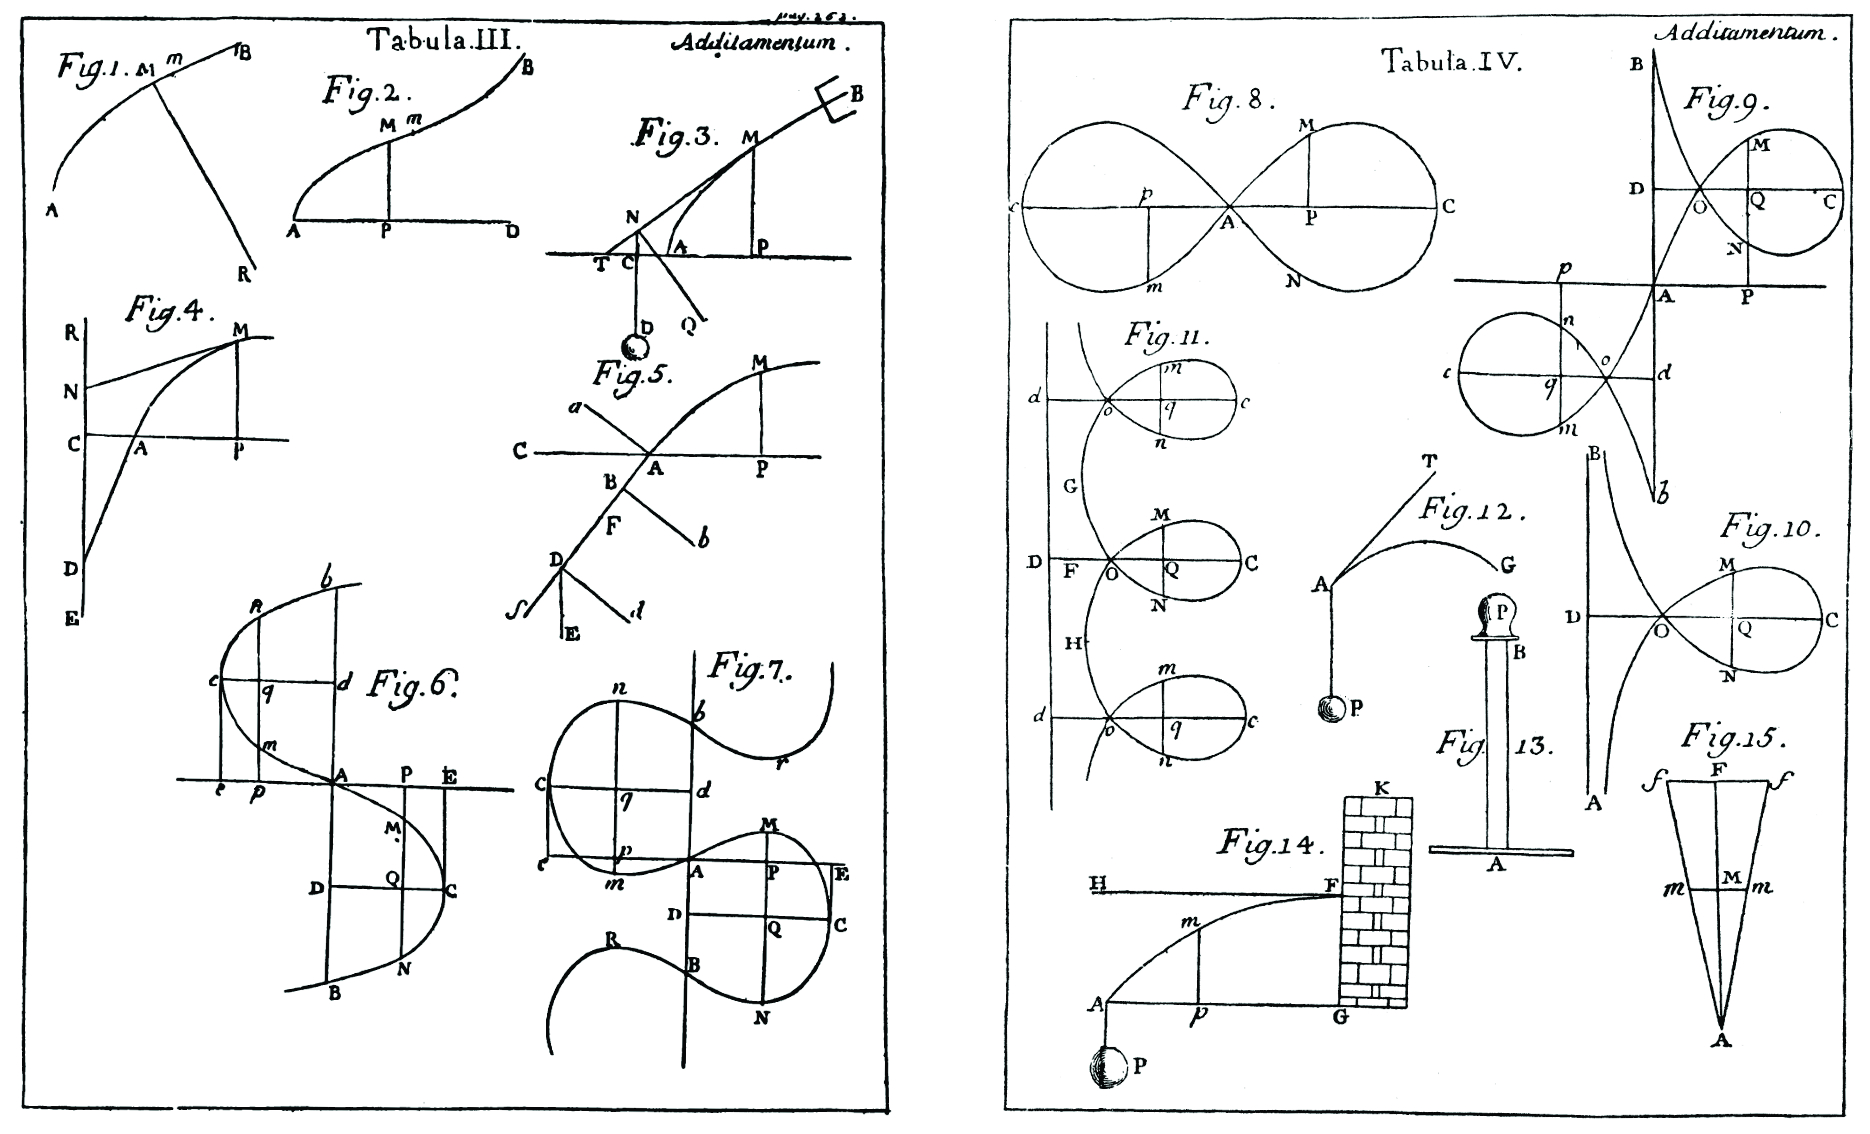
\includegraphics{partes/figs/euler.jpg}}
	\end{center}
	\titfigura{Different configurations of the elastic band on Euler's \emph{De Curvis Elasticis}.}\label{fg:euler}
\end{figure}     
Concerning the problem proposed by Bernoulli for bands of uniform elasticity and cross section, represented on drawing 1 of tabula III, the elastic potential $\int ds/{r^2}$ is described by $\int Zdx$ on rectangular coordinates, where $Z={q^2}/{\sqrt{(1+p^2)^5}}$, $p=dy/dx$ and $q=dp/dx$. Through some development he did not present, Euler stated that finding the minimum of $\int Zdx$ is the same as solving the equation
\begin{equation*}
\dfrac{d^2Q}{dx^2} - \dfrac{dP}{dx} + \alpha \dfrac{d}{dx}(\dfrac{p}{\sqrt{1+p^2}}) = 0\,,
\end{equation*}
where $Q=d Z/d q$, $P=d Z/d p$ and $\alpha$ is a constant. Integrating this differential equation, we can write that
\begin{eqnarray*}
\dfrac{dQ}{dx} - P +  \dfrac{\alpha p}{\sqrt{1+p^2}} = \beta&\text{or}&\dfrac{dQ}{dp}q - \dfrac{dZ}{dp} +  \dfrac{\alpha p}{\sqrt{1+p^2}} = \beta
\end{eqnarray*}
because ${dQ}/{dx}={dQ}/{dp}.{dp}/{dx}$. Integrating again and isolating $q$, we arrive at 
\begin{equation*}
q = \dfrac{1}{Q}(\beta p + \gamma + Z -\alpha\sqrt{1+p^2})\,.
\end{equation*}
Since $q={dp}/{dx}={dp}/{dy}.{dy}/{dx}=p\cdot{dp}/{dy}$, then
\begin{eqnarray*}
\dfrac{dp}{dx}= (1+p^2)^{\frac{5}{4}} \sqrt{\alpha\sqrt{1+p^2}+\beta p + \gamma} &\text{and}& \dfrac{dp}{dy}= \dfrac{1}{p}\dfrac{dp}{dx}\,.
\end{eqnarray*}
At this point, since $({du}/{dv})^{-1}={dv}/{du}$, Euler made use of the so called mathematical sagacity to construct the equality 
\begin{equation*}
\beta \dfrac{dx}{dp} - \gamma \dfrac{dy}{dp} = \dfrac{(\beta-\gamma p)}{(1+p^2)^{\frac{5}{4}} \sqrt{\alpha\sqrt{1+p^2}+\beta p + \gamma}}
\end{equation*}
whose integration leads to 
\begin{equation}\label{eq:euler1}
\beta x - \gamma y + \delta = \dfrac{2\sqrt{\alpha\sqrt{1+p^2}+\beta p + \gamma}}{\sqrt[4]{1+p^2}}\,.
\end{equation}
Then he proceeded a change of variables by rotating and translating the orthogonal axes in such a way that               
\begin{eqnarray*}
X= \dfrac{\beta x - \gamma y+\delta}{\sqrt{\beta^2+\gamma^2}} &\text{and}& Y= \dfrac{\gamma x + \beta y+\delta}{\sqrt{\beta^2+\gamma^2}}\,.
\end{eqnarray*}
From these equalities and considering $\tilde{p}={dY}/{dX}$, it is possible to write that
\begin{align*}
p &= \dfrac{d}{dx}(\dfrac{Y\sqrt{\beta^2+\gamma^2}-\gamma x +\delta}{\beta})\\
&= \dfrac{1}{\beta}(\dfrac{dY}{dX}\dfrac{dX}{dx}\sqrt{\beta^2+\gamma^2}-\gamma)\\
 &= \dfrac{1}{\beta}[\tilde{p}(\beta-\gamma p)-\gamma]\\
&= \dfrac{\beta\tilde{p}-\gamma}{\beta+\tilde{p}\gamma}
\end{align*}
and also that $1+p^2 = (\beta^2+\gamma^2)(1+\tilde{p}^2)/(\beta+\gamma\tilde{p})^2$. Substituting all these values on \eqref{eq:euler1}, Euler obtained that
\begin{equation*}
X\sqrt{\beta^2+\gamma^2} = \dfrac{2\sqrt{\alpha\sqrt{1+\tilde{p}^2}+ \tilde{p}\sqrt{\beta^2+\gamma^2}}}{\sqrt[4]{1+\tilde{p}^2}}
\end{equation*}
and considered $\beta_1=\sqrt{\beta^2+\gamma^2}$, which led to $X\beta_1\sqrt[4]{1+\tilde{p}^2} = 2\sqrt{\alpha\sqrt{1+\tilde{p}^2}+ \tilde{p}\beta_1}$. Generically, this last result can be rewritten as 
\begin{equation*}
x\beta\sqrt[4]{1+p^2} = 2\sqrt{\alpha\sqrt{1+p^2}+ p\beta}\,.
\end{equation*}
From this equation, through algebraic manipulations, he arrived at
\begin{equation*}
p=\dfrac{n^2x^2-ma^2}{\sqrt{n^2a^4-(n^2x^2-ma^2)^2}}
\end{equation*}
where $m=\alpha a^2/4$ and $n=\beta a^2/4$. Making a new change of variables where $n=k$, $x=\tilde{x}+c/2k$ and $m=a^{-2}(c^2/4-bk)$ and developing the previous equation, he finally obtained the deflection equation  
\begin{equation}\label{eq:dflect}
\dfrac{dy}{dx}=\dfrac{(b+c x+k x^2)}{\sqrt{a^4-(b+c x+kx^2)^2}}
\end{equation}
of the \emph{elastica} with each of its fixed endings submitted to a given couple; confirming the result already obtained by Jakob Bernoulli in 1695 through an approach which Euler called \emph{a priori} method (causes) instead of Daniel's method of maxima and minima (effects). In order to prove the generality of his result, Euler solves through an \emph{a priori} method the configuration of the \emph{elastica} presented on drawing 3 of tabula III, that is, with an ending fixed and the other attached to a rigid staff subjected to a load $P$. In this context, from a paper published by Daniel Bernoulli in 1728, in which he stated that the moment $Px=EI\kappa$, where $x$ is the distance of the section from the applied load, $E$ is the Young's modulus, $I$ a geometrical quantity (known today as the moment of inertia) and curvature 
\begin{equation*}
\kappa=\dfrac{d^2y/dx^2}{[1+({dy}/{dx})^2]^{3/2}}\,,
\end{equation*}
Euler obtained the equation
\begin{equation*}
\dfrac{dy}{dx}=\dfrac{-P(b+c x+x^2/2)}{\sqrt{E^2I^2-P^2(b+c x+x^2/2)^2}}\,,
\end{equation*}
which is compatible to \eqref{eq:dflect} and valid for large elastic deflections. When small deflections are considered, the curvature $\kappa \approx d^2y/dx^2$ and then the deflection equation results $d^2y/dx^2=Px/EI$. In tabulae III and IV, Euler analyzes other forms of the \emph{elastica} and also the strength of a column to buckling: considering drawing 13, he states that a column with uniform cross section will not bend if $P\leqslant EI(\pi/h)^2$, where $h$ is its height.        

In 1817, the French civil engineer Augustin-Louis Cauchy (1789-1857) was in charge of the disciplines of Mechanics and Analysis at the \'Ecole Polytechnique in Paris and, from Euler's concept of hydrostatic pressure $p$ in a perfect fluid, he taught his students that the property of $p$ being the same in all directions was a consequence of its perpendicular action on the surfaces involved\footnote{See \aut{Belhoste}\cite{belhoste_1991_1}, p. 92.}. At Facult\'e des Sciences, also in Paris, where he lectured on Mechanics and Mathematics by the year of 1821, he began extending his ideas on hydrostatics to any deformable body. Already established as a renowned mathematician, Cauchy was frequently considered by some fellows in French scientific circles to be the special recipient of their work: in a letter dated July 24, 1821, he acknowledged the mathematician Marie-Sophie Germain (1776-1831) for having sent him \emph{Research on the Theory of Elastic Plates}, published that same year, a work in which she solved a mathematical problem concerning vibration of elastic surfaces and that had already made her the winner of a competition organized by the Paris Academy of Sciences in 1816. Inspired by this work and the ideas of Augustin-Jean Fresnel (1788-1827) and Claude-Louis Navier (1785-1836), which were also working on mathematical models for the mechanical behavior of deformable bodies, Cauchy managed to anticipate these two renowned scholars and published in 1823 an abstract entitled \emph{Researches On The Equilibrium And Internal Motion Of Solid Bodies Or Fluids, Elastic Or Non-elastic} on the January edition of the \emph{Bulletin of the Soci\'et\'e Philomatique}, which was submitted on September 30 of the previous year. Read out loud by Cauchy himself on a meeting of the Soci\'et\'e Philomatique in February 22, 1823, the abstract delineated the concept of stress, which he adapted from Euler's hydrostatic pressure, and its implications. The great relevance of this abstract as a document attesting the birth of the modern approach to Continuum Mechanics, which is the last period of our brief history, is the reason why we allow ourselves to reproduce it completely, as follows, in our English translation of the original text by \aut{Cauchy}\cite{cauchy_1823}.

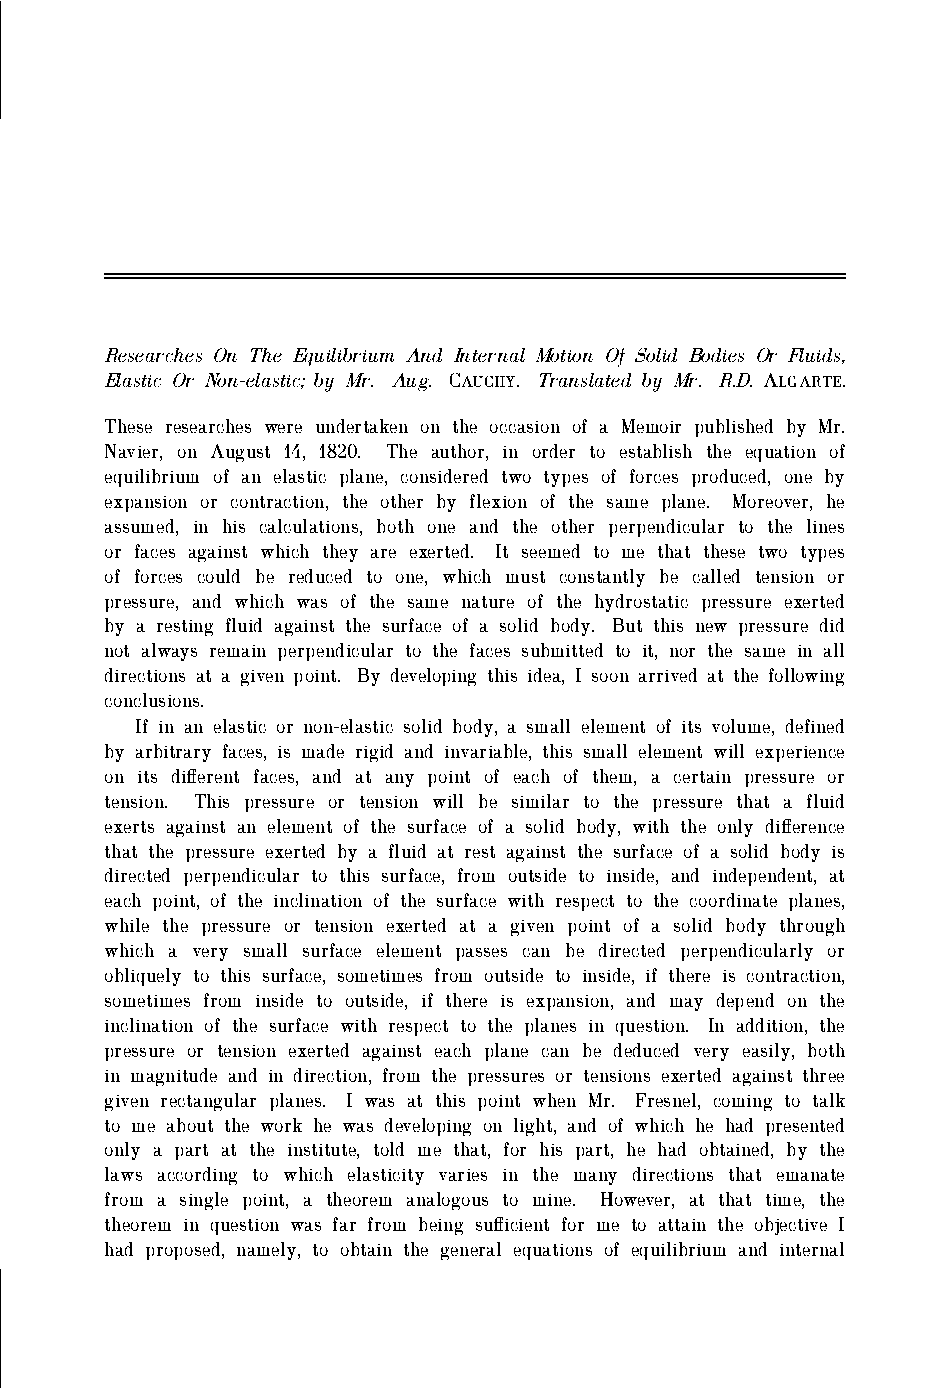
\includepdf[pages=-]{partes/parte2/c_cauchy.pdf}

Since there are very few reliable sources of Cauchy's biography, we shall mostly rely on the definitive account of \aut{Belhoste}\cite{belhoste_1991_1}. Born in Paris in August 21, 1789, one month after the Storming of the Bastille, which marked the effective breakout of the French Revolution, Cauchy was the eldest of the six children of Louis-Fran\c{c}ois Cauchy, a highly ranked senior official of the French Senate, and Marie-Madeleine Desestre, a middle-class Parisienne whose most of the relatives, including her father and brother, occupied lower posts in the Parisian government. At the time of Cauchy's birth, Louis-Fran\c{c}ois had a post at the police of Paris and was closely related to Lieutenant G\'eneral Louis Thiroux de Crosne, his benefactor. When Thiroux, returning from England, was arrested and beheaded in April 28, 1794, by the revolutionary authorities, Louis-Fran\c{c}ois hasted to flee from Paris with his wife and two sons, the five-year-old Augustin-Louis and the baby Alexandre-Laurent, to live in the commune of Arcueil, in a country house they had bought years before. There,  the eldest son not only contracted smallpox but also received the first lessons on elementary education from his father, who had been a brilliant Law student at the University of Paris. After the execution of Robespierre in July 27 and the fall of his followers, the widespread turmoil ceased: arrests and executions decreased substantially; the overall conditions improved, which led to the end of the so called Reign of Terror. Since there were no more reasons to fear political persecution, the Cauchys returned to Paris that same year, and Louis-Fran\c{c}ois assumed an administrative post at the Ministry of Interior in Autuum. A fervent supporter of the ideas, plans and political movements that conduced Napoleon Bonaparte to power as the First Council of France in November 1799, following the coup d'etat of 18 Brumaire, Louis-Fran\c{c}ois was rewarded in January 1800 with the position of Secretary-General at the newly created Senate, a highly prestigious post, inferior only to that of Chancellor, which was occupied at that time by senator Pierre-Simon Laplace (1749-1827), the famous polymath. As the Secretary-General of the Senate, Louis-Fran\c{c}ois had obviously to be in daily contact with many senators, an interaction that eventually ended in friendship, as was the case with Chancellor Laplace and senator Joseph-Louis Lagrange (1736-1813). Already informed by Louis-Fran\c{c}ois about the skills and interests in Mathematics of the young Augustin-Louis, the renowned Italian-French mathematician, senator Lagrange, is said to have given the following piece of advice to his friend Louis-Fran\c{c}ois: ``\emph{Do not allow him even to open a Mathematics book nor write a single number before he has completed his studies in literature}''. And so it was done: under Lagrange influence and conduction, Augustin-Louis entered the \'Ecole Centrale du Panth\'eon in 1802 to course Latin and humanities. However, during this period, he performed brilliantly and won many competitions in ancient languages, graduating two years later with distinction. Despite this success in humanities, Augustin-Louis ended up breaking the family tradition of studying Law in order to satisfy his early interests in Mathematics and then decided to enroll the \'Ecole Polytechnique the following year of 1805 to become an engineer of the French public service. But this surprising decision did not exasperate Louis-Fran\c{c}ois, who provided all the necessary material support and also took advantage of his great prestige to enable the success of his son's career. Examined by the renowned mathematician Jean-Baptiste Biot (1774-1862), among 293 applicants, Augustin-Louis ranked the second place out of 125 approved, and chose to specialize in highways and bridges, the area in the public service where he would work after finishing the course. Among the disciplines at \'Ecole Polytechnique, he attended classes on Algebra by Jean-Guillaume Garnier (1766-1840), Calculus by Sylvestre Lacroix (1765-1843), Geometry by Gaspard Monge (1746-1818) and Mechanics by Gaspard de Prony (1755-1839); with the tutorship of Andr\'e-Marie Amp\`ere (1775-1836). Augustin-Louis performed accordingly on these fundamental disciplines, which constituted the first two years of the course. After this period, he entered the \'Ecole des Ponts et Chauss\'ees at the end of 1807, in order to specialize in highways and bridges, as he had chosen. In the spring of 1808, he joined the team of the Ourcq Canal project, under the supervision of Pierre-Simon Girard (1765-1836), as a practical discipline of the course. In January 1810, he graduated with distinction as a junior engineer and, in February, was sent to work in the construction of Port Napoleon, in Cherbourg. The job was very demanding but Augustin-Louis kept developing his studies on pure Mathematics, particularly Geometry. In this period, he submitted \emph{Studies on polyhedra} in 1811 to the \emph{Journal de L'\'Ecole Polytechnique}, an article that was highly praised by the judging commission and that brought him a good recognition in Paris. However, Augustin-Louis suddenly found himself drained by the obligations of a job he clearly hated and also very anxious by the opportunities he might be losing of pursuing an academic career on pure science in the capital. Endowed with the typical psychological rigidity that stems from a strong religious education, he could not manage his frustrations and got deeply depressed. In September 1812, when Marie-Madeleine went to visit Augustin-Louis in Cherbourg, she saw her son in a very bad condition and quickly took him back to Paris, definitely. After recovering from his illness, he kept studying Mathematics and finished two papers: one of them on the theory of combinations and the other on the theory of determinants, both submitted to the \emph{Journal de L'\'Ecole Polytechnique} and accepted. In order not to be sent back to Cherbourg, Augustin-Louis resorted to his father's prestige and influent friends to stay in Paris, when he was appointed to a post of engineer at the Ourcq Canal, a place he already known. While working there, his paper \emph{On Definite Integrals}, submitted to the  \'Ecole Polytechnique in August, 1814, was highly praised and in December he was elected member of the Soci\'et\'e Philomatique de Paris. On November, 1815, favorable political conditions led the Governor of the \'Ecole Polytechnique to appoint Augustin-Louis assistant professor of Analysis, replacing the sickly professor Louis Poinsot (1777-1859). In this same month, he presented a study that would make him internationally famous, \emph{Proof of Fermat's General Theorem on Polygonal Numbers}, published as an appendix of a Legendre's paper in 1816. This sudden notoriety enabled him to apply for a membership at the famous Royal Academy of Sciences and in March, 1816, Louis XVIII surprisingly appointed the twenty-seven-year-old Cauchy a member of the academy, replacing Gaspard Monge, expelled for political reasons. The reactionary political trend in France in that period and the great influence of his highly conservative father would once more favor Augustin-Louis' academic pretensions: in June he was appointed for full professorship in Analysis and Mechanics at the \'Ecole Polytechnique. He also started teaching as an eventual substitute professor at the Coll\`ege de France and at the Facult\'e des Sciences. In April 4, 1818, Cauchy married to Alo\"ise de Bure, member of a traditional family of publishers and booksellers; a condition that later on proved to be quite convenient because it enabled him to publish most of his works independently, with the help of his father-in-law, on a periodical called \emph{Exercices de Math\'ematiques}, dedicated only to his works. He and Alo\"ise had two daughters, Marie Fran\c{c}oise Alicia, born in 1819, and Marie Mathilde, born in 1823. In 1821, he published the first part of \emph{Cours D'Analyse}\footnote{For an English translation, see \aut{Bradley \& Sandifer}\cite{bradley_2009}.}, called \emph{Analyse Alg\'ebrique}: a seminal textbook that, for the first time, presented infinitesimal calculus in a rigorous mathematical approach. It was in this context that Cauchy started developing and presenting his theories on Fluid and Solid Mechanics, which led to the submission of the aforementioned abstract on the equilibrium of deformable bodies in September, 1822. After the publication of this abstract in January, 1823, Navier correctly claimed that his August 1820 paper, cited by Cauchy in the abstract, had still not been published and waited for evaluation by the commission of Soci\'et\'e Philomatique together with another paper of his, \emph{On the Laws of Equilibrium and Motion of Elastic Solid Bodies}, submitted in May, 1821, that covered the same subject of Cauchy's abstract. Rumors of plagiarism began to be heard and then Augustin-Louis decided not to publish his achievements. This whole uncomfortable affair was the main reason for him to start publishing the mathematical development of his equilibrium equations only four years later, after Navier published his own paper on the January 1827 edition of the \emph{M\'emoires de L'Acad\'emie des Sciences de L'Institut de France}. During this delay, Cauchy made improvements on the theory and on its mathematical developments, which resulted in four papers published on his personal periodical \emph{Exercices de Math\'ematiques} in the following chronological order. 
\begin{itemize}
	\setlength\itemsep{1pt}
	\item[1.] March, 1827, pp. 42-57: \emph{Sur La Pression ou Tension Dans Les Corps Solides}\footnote{See \aut{Cauchy}\cite{cauchy_1827}. In Appendix A, p. \pageref{ch:appA}, I translated to English a newer version of this paper.} (On the Pressure or Tension in Solid Bodies);
	\item[2.] April, 1827, pp. 60-69: \emph{Sur La Condensation Et La Dilatation Des Corps Solides} (On the Contraction and Expansion of Solid Bodies);
    \item[3.] April, 1827, pp. 108-111: \emph{Sur Les Relations Qui Existent, Dans L'etat D'equilibre D'un Corps Solide Ou Fluicie, Entre
les Pressions Ou Tensions Et Les Forces Acceleratrices} (On The Relations That Exist, in the State of Equilibrium of a Solid or Fluid Body, Between the Pressures or Tensions and the Accelerating Forces);
	\item[4.] September, 1828, pp. 160-187: \emph{Sur Les Equations Qui Expriment Les Conditions D'equilibre Ou Les Lois Du Mouvement interieur D'un Corps Solide, Elastique Ou Non Elastique} (On the Equations That Express the Conditions of Equilibrium or the Laws of Interior Motion of a Solid Body, Elastic or Non-elastic).
\end{itemize}
The first of these important works became a classic on the emerging field of Continuum Mechanics, where Cauchy developed the subject presented on the abstract of 1823, and the others were improvements of the topics presented in this first one. Meanwhile, he also published in the March 1826 edition of his personal periodical the article \emph{A New Genre of Calculus Analog to Infinitesimal Calculus}, where he presented the decomposition of rational fractions by means of the calculus of residues. A complex function of a complex variable was defined for the first time in the textbook \emph{Lessons on Differential Calculus}, which he published in 1829, a year that closed a cycle of the greatest productivity in Cauchy's career; the political turmoil of the following period would definitely misguide him. Since the fall of Napoleon in 1814, France had been watching a strong political conflict between the supporters of the constitutional monarchy, led by the Bourbon monarch Charles X, and the bourgeois liberal movement. After the elections of 1830, when the liberals took the majority in the Chamber, the monarchy tried to suspend the freedom of the press and to dissolute the parliament. As a result, the so called Second French Revolution broke out in July 26, 1830, which led to the overthrow of Charles X by his cousin Louis Philippe, from the House of Orl\'eans. Enraged by this profound political transformation that ended with the fall of the regime the Cauchys had passionately supported for so long and also by the oaths that he, as a public server, would have to make for the new king, the anti-liberal and impulsive Augustin-Louis Cauchy, falsely claiming health issues, left all his job positions and his country to the Italian city of Turin in the beginning of September 1830, a trip he imagined would not be so long -- since his wife and daughters stayed in Paris -- as it really turned out to be. Still abroad in November of that same year, the claim of health problems was no longer convincing and then he lost the position at Facult\'e des Sciences; in January 1831, he was fired from \'Ecole Polytechnique and also from the engineering post at Ponts et Chauss\'ees in March, but he managed to keep his membership at the Royal Academy. In Turin, the King Charles Albert of Sardinia created a post of Physics professor at the University specially for the famous French mathematician, a position Cauchy held from 1832 to 1833. In August 1833, he left Turin to Prague in order to be the tutor of the thirteen-year-old Duke of Bordeaux, the exiled grandson of Charles X. One year later, his  wife and daughters finally came to live with him after four years apart. The unsuccessful and troublesome tutorship lasted until 1838, a period after which he received the title of baron from Charles X. Cauchy returned to Paris in the autumn of 1838 and resumed his activities only at the Academy since he still refused to swear loyalty to the king, a mandatory requirement for French professors at that time. In 1843, he applied for a vacant chair of Mathematics at the Coll\`ege de France, but was not approved mainly for political reasons, since he was engaged in reestablishing the prestige of catholic university education in Paris, a movement considered by the academic community to be contrary to the Enlightenment ideals. With the fall of King Louis Philippe, the rise of Louis Napoleon Bonaparte in 1848 as the president of the French republic and the abolition of the oath requirement for public servers in 1849, Cauchy got a post of professor of mathematical astronomy at Facult\'e de Sciences, where he worked until the end of his life. In May 12, 1857, under his doctor's advice, Cauchy left Paris to his country house in Sceaux, in order to spend the whole summer, as a treatment for his unknown illness, but in May 23, at 4 a.m., ``\emph{he met death with such a calm that made us ashamed of our unhappiness}''\footnote{See \aut{Belhoste}\cite{belhoste_1991_1}, p.240.}, wrote his daughter Alicia. 

Leonhard Euler starts the first volume of his fundamental \emph{Scientia Navalis} with a lemma stating that \emph{``The pressure which the water exerts upon a submerged body in its several points is normal to the surface of the body; and the force which an arbitrary element of the submerged surface sustains is equal to the weight of a right aqueous cylinder whose base is equal to the element of surface itself, and whose altitude is equal to the depth of the element below the upper surface of the water.''}\footnote{\aut{Euler}\cite{euler_1749_1}, p. 1, translated from the Latin by \aut{Truesdell}\cite{truesdell_1954_1}.} The property of normal punctual compressions on surfaces submerged in water at rest was already known in 1738 and, according to \aut{Truesdell}\cite{truesdell_1954_1}, it is difficult to trace its origins. It was also known the idea of considering the weight of the water sustained by a submerged surface analog to sustaining a column of water, which was first presented by the Belgian engineer Simon Stevin (?-1620) on his work \emph{Hypomnemata mathematica: De statica}, published in 1605. Today, these properties of water are assigned to a group of fluids called perfect, which have the feature of being ``slippery'', not capable of resisting tangential (shear) forces. In addition to the clarity and simplicity of a mathematical text, what is brilliant in Euler's statement is his new concept of pressure (punctual compression) as a measure of force per unit of area on each point of the submerged surface. Inspired by this concept of pressure and its corollaries, Cauchy came up with the idea that an element in the interior of a solid body has its surfaces also subjected to pressures, but, unlike the case of a perfect fluid at rest, a pressure on an arbitrary point of a solid surface may not be normal and may not be positive (compressive).  In his \emph{Sur La Pression ou Tension Dans Les Corps Solides}, from a small volume of solid limited by infinite surfaces with boundaries, Cauchy considered a pressure or tension (negative pressure) $p_i$ acting on the points of an arbitrary surface $s_i$, defined $(\cos\lambda_i,\cos\mu_i,\cos\nu_i)$ as the cosine directions of $p_i$ relative to rectangular coordinate axes $(x,y,z)$ and took plane $xy$ as a reference to describe the components of forces
\begin{eqnarray*}
\iint p_i\cos\lambda_i\sec\gamma_i\,dxdy\,, \quad \iint p_i\cos\mu_i\sec\gamma_i\,dxdy &\text{and}& \iint p_i\cos\nu_i\sec\gamma_i\,dxdy\,,
\end{eqnarray*}
where $\gamma_i$ defines the cosine direction relative to $z$ of the unit normal to $\sec\gamma_i\,dxdy$, which is an infinitesimal element of $s_i$. When the volume of the small element tends to zero, higher order terms become negligible, and the above integrals are respectively simplified to        
\begin{eqnarray*}
p_iA_i\cos\lambda_i\,, \quad p_iA_i\cos\mu_i  &\text{and}& p_iA_i\cos\nu_i\,,
\end{eqnarray*}
where $A_i$ is the area of $s_i$. Concerning the infinite surfaces of the volume element in equilibrium, the balance of all the forces involved results
\begin{eqnarray*}
\sum_{i=1}^\infty p_iA_i\cos\lambda_i=0\,, \quad \sum_{i=1}^\infty p_iA_i\cos\mu_i=0 &\text{and}& \sum_{i=1}^\infty p_iA_i\cos\nu_i=0\,.
\end{eqnarray*}
Cauchy applies this same procedure for linear momenta relative to the coordinate axes and obtains their correspondent balance expressions. Then, he considers a small volume element with the shape of a right prism whose bases $s_1$ and $s_2$ are parallel to the plane $xy$, both having area $A$. Making this prism infinitesimal by decreasing its height faster than the sides of its bases, this height can be neglected and therefore what remains of the element is an infinitesimal plane of area $dA$ with faces labeled $ds_1$ and $ds_2$. In this context, the previous balance of forces can be described by  
\begin{eqnarray*}
\sum_{i=1}^2 p_idA_i\cos\lambda_i=0\,, \quad \sum_{i=1}^2 p_idA_i\cos\mu_i=0 &\text{and}& \sum_{i=1}^2 p_idA_i\cos\nu_i=0\,,
\end{eqnarray*}
from which equalities $p_1=p_2$, $\cos\lambda_1=-\cos\lambda_2$, $\cos\mu_1=-\cos\mu_2$ and  $\cos\nu_1=-\cos\nu_2$ can be concluded. Although simple, this result is fundamental in Cauchy's mechanical theory because it allows us to assert that \emph{an arbitrary infinitesimal  plane, to which a point in equilibrium belongs, defines on it a unique pair of opposing tensions or pressures with the same intensity}. Making a small parallelepiped in equilibrium an infinitesimal volume element, a consequence of the previous statement is that, among the six pressures or tensions on the element faces, only three may be distinct, namely $p_1$, $p_2$ and $p_3$. In this context, Cauchy then obtains from the balance of linear momenta that tangential pressures or tensions $p_1\cos\mu_1=p_2\cos\lambda_2$, $p_1\cos\nu_1=p_3\cos\lambda_3$ and $p_2\cos\nu_2=p_3\cos\mu_3$. 

Considering the set of all deformable bodies as constituted by solids and fluids, the feature of an arbitrary plane defining a pair of opposing pressures or tensions on a point in equilibrium becomes a generalization of the particular case of perfect fluids at rest, where an arbitrary plane, to which a point of depth $h$ belongs, defines on it a pair of opposing equal pressures normal to this plane (hydrostatic). Moreover, if we represent tensions or pressures by geometric vectors and consider the general case of deformable bodies, the set of all the planes to which a point in equilibrium belongs defines on it a set of vectors that may not constitute a sphere, as does the set of all hydrostatic pressures on a point inside a perfect fluid at rest, since the intensity of an hydrostatic pressure depends only on the depth $h$, according to Euler's lemma. If the geometric shape of the set of tension or pressure vectors on a point in equilibrium may not be a sphere, which shape would it be? In order to answer this question, Cauchy elects his famous tetrahedron as a small volume element, defines pressure $p$ on a point of its basis $s$ as unknown and $(\cos\alpha,\cos\beta,\cos\gamma)$ as the cosine directions of the unit normal to $s$. From the previous expressions of balance of forces and after lengthy algebraic manipulations, he arrives at the following equations:
\begin{align*}
p^2 = &(\text{A}\cos\alpha+\text{F}\cos\beta+\text{E}\cos\gamma)^2+\\
&(\text{F}\cos\alpha+\text{B}\cos\beta+\text{D}\cos\gamma)^2+\\
&(\text{E}\cos\alpha+\text{D}\cos\beta+\text{C}\cos\gamma)^2
\end{align*}
and the projection of tension or pressure $p$ on the unit normal to $s$ 
\begin{align*}
p\cos\delta &= \text{A}\cos^2\alpha+\text{B}\cos^2\beta+\text{C}\cos^2\gamma+\\
&+2\text{D}\cos\beta\cos\gamma +2\text{E}\cos\gamma\cos\alpha+2\text{F}\cos\alpha\cos\beta\,
\end{align*}
where coefficients $\text{A} = p_1\cos\lambda_1$, $\text{B} = p_2\cos\mu_2$, $\text{C} = p_3\cos\mu_2$, $\text{D} = p_2\cos\nu_2$, $\text{E} = p_3\cos\lambda_3$ and $\text{F} = p_1\cos\mu_1$. Relative to the point on which it acts on $s$, the vector defined by $p\cos\delta$  has coordinates $\text{x}=p\cos\delta\cos\alpha$, $\text{y}=p\cos\delta\cos\beta$ and $\text{z}=p\cos\delta\cos\gamma$. Considering these coordinates, the previous equality divided by $(p\cos\delta)^2$ results the polynomial 
\begin{equation*}
\text{A}\text{x}^2+\text{B}\text{y}^2+\text{C}\text{z}^2+2\text{D}\text{y}\text{z} +2\text{E}\text{z}\text{x}+2\text{F}\text{x}\text{y}- \dfrac{1}{p\cos\delta} = 0\,,
\end{equation*}  
which represents an ellipsoid. Cauchy then found out that there is a particular base $s$ of the tetrahedron to which $p$ is normal and all tangential pressures or tensions vanish. In other words, $\cos\delta=1$, $\cos\nu_2=\cos\lambda_3=\cos\mu_1=0$ and as a straightforward consequence $\cos\lambda_1=\cos\mu_2=\cos\nu_3=1$, from which we conclude that $p_1$, $p_2$ and $p_3$ are normal to their respective planes. He called these values principal pressures or tensions and, among them, there is the maximum and the minimum values of all the pressures or tensions on the point under consideration. In this context, we can rewrite the previous polynomial as following:
\begin{eqnarray*}
1 &=& p\text{A}\text{x}^2+p\text{B}\text{y}^2+p\text{C}\text{z}^2 \\
&=& p_1^3p^3\cos^2\alpha/p_1^2 + p_2^3p^3\cos^2\beta/p_2^2+p_3^3p^3\cos^2\gamma/p_3^2\\
&=& X^2/p_1^2 + Y^2/p_2^2 + Z^2/p_3^2\,,
\end{eqnarray*} 
from which it is clear that the principal pressures or tensions define the magnitutes of the axes of the ellipsoid. This result justifies the fact that today we also call the planes defined by the axes of the ellipsoid as principal.

 


